\newpage

\section{\MakeUppercase{Mitchell Innes versus Other Creditists}}\label{sec:other_creditists}

%\subsection{\capitalizetitle{Mitchell Innes versus other creditists}}\label{sec:other_creditists}

\subsection{Introduction}

Available literature on the contribution of \citeauthor{innes1913} to monetary economics is limited. He was re-discovered by the contemprory heterodox economists about in the end of 1990s. What was discussed in Chapter~\ref{sec:innes} is rather new and was not covered in due respect yet. Current Chapter~\ref{sec:other_creditists} discusses major creditists, the term borrowed from \cite{earley1994}, such as Keynes, Schumpeter, and Minsky. Also, writings by \citeauthor{commons1951} and \citeauthor{colwell1860} deserve attention: the former is renowned as major contributor to traditional institutionalism, the latter wrote a book on payments in the middle of nineteenth centtury after carrying out an analysis of the European credit system.

Overall, thic chapter attempts to find correspondence of these economists' analysis of money and monetary economics with that of \citeauthor{innes1913}. In particular, it pays special attention towards the writings, which are close to the latter's essential ideas highlighted in the section \ref{sec:essential}, p.~\pageref{sec:essential}.

\begin{figure}[!ht]\centering
\includegraphics[width=1.0\textwidth]{\plotsfolder/econs_lives}
\caption[Selected economists writing on the credit theory and credit system practice]%
{Selected economists writing on the credit theory and credit system practice: life spans and timing of major works\par \small Red lines indicate years, when major works by the named creditists were published: see \cite{colwell1859,colwell1860}, \cite{innes1909,innes1910,innes1913,innes1914,innes1914a,innes1932}, \cite{keynes1930a,keynes1936}, \cite{schumpeter1934,schumpeter1939_1,schumpeter1968,schumpeter2014}, \cite{minsky1975,minsky1986}.
}
\end{figure}

%
% -------------- Stephen Colwell (1800-1871) -----------------------------------+
%
\subsection{Stephen Colwell}\index{Colwell, Stephen}

In the United State of mid 19th century, a book titled \textit{The Ways and Means of Payment} was published by Philadelphia-based publisher. It was authored by \citeauthor{colwell1859} (1800-1871), an industrialist from Philadelphia and member of the local elite. See \citep{colwell1859}. 

The author ``had considerable abilities as an economic thinker. \dots  In the 1850s Colwell authored numerous books and articles on topics ranging from the state of manufacturing in Pennsylvania, to the national credit system" \citep[chapter~8, pp.~109-121]{davenport}. 

His biography accounts reveal him as a person, who was an impatient learner of social and economic relations. At the age of thirty six, he started running his father-in-law iron manufacturing business. This took place upon his return from Europe, where he traveled by the insistence of father-in-law to study the state-of-the-arts methods and practices of the local industrialists. He visited England, being attracted to observe firsthand its productive capacities in the midst of Industrial Revolution. In addition, he visited France, Sweden and Belgium \citep[footnote 3, p.~235]{davenport}. He picked up from that learning trip a number of observations that impacted him intellectually. Some accounts mention his dissatisfaction with the observed plight of the working people in the most advanced industrialist lands. He read the works of Adam Smith and critically reviewed his ideas in own writings. His curiosity in the changing world made him great collector of books on the subject of banking and general political economy thought. Upon his death, his personal library consisting of about six thousand titles was handed over to the University of Pennsylvania \citeyearpar[p.~110]{davenport}. He strived to influence the way Americans think of economic matters. In addition to own publications, it appears that he put effort to make the works of German economist Friedrich List published in the United States: the same Philadelphia-based publisher that in 1859 published Colwell's payments book in 1856 published \citeauthor{flist1856}'s major work \textit{National System of Political Economy}. \cite[footnote 12, p.~380]{breton1964} mentioned Colwell as translator of the List's book. Indeed, Colwell favorably viewed the writings of the German economist to such an extent that he wrote an extensive introductory essay to that book, see \citep{colwell1856}. \citeauthor{colwell1859}'s own major work on the subject of political economy was the above-mentioned \textit{The Ways and Means of Payment}, see \citeyearpar{colwell1859}. It became ``his finest treatise" \citep[p.~819]{dorfman2}:    

\begin{quote}
Into its 644 pages Colwell poured a large part of the contents of his vast library on the literature of banking.~\citep[p.~819]{dorfman2}
\end{quote}

A condensed version of the book was put into an article, which was published a year after  \citep{colwell1860}. Indeed, at the time, this book was considered ``the most impressive single work on banking produced in America before 1860" \citep[p.~494]{selgin1989}. 

In this book, \cite{colwell1859,colwell1860} explains the efficiency of the commercial activities as those were utilizing the ``Credit system." For \citeauthor{colwell1859}, the latter epitomized a state of the art system, hence, he referred to it by capitalizing the word credit. He perceived it as being developed from the method of paying with precious meal coins, which was seen as traditional and hence easily and widely recognized. Then, the ``Credit system" detached itself from the ordinary way of payments. His experience with European methods of commerce made him aware of enomous disproportions between payments done through the ``Credit system" and those done with precious metal coins.

\begin{quote}
As more than nine-tenths of all the payments of trade are effected 
without the intervention of gold or silver, it becomes proper to ascertain 
the way in which this large proportion of payments is effected. \dots 
How, then, are the payments chiefly made in the commercial world?~\citep[p.~685]{colwell1860}
\end{quote}

His own research on the payments provided him with the followed brief exposition as an answer:

\begin{quote}
Credits and debts are counterparts -- that is, there being two parties to each debt and 
credit, one is always a debtor and the other always a creditor.~\citep[p.~688]{colwell1860}
The credit system is that by which men set-off\index{Colwell, Stephen!on set-off} the debts wlich others owe them against those which they owe to others.~\citep[p.~8]{colwell1859} 
\end{quote}

In a broad extent, the terminology and its meaning used \citeauthor{colwell1859} was quite similar to \citeauthor{innes1913} as far as technique of payment is concerned.\footnote{For example, compare \citeauthor{colwell1859}'s ``[e]ach individual, in fact, directly or indirectly pays for what he purchases with that which he has to sell"~\citep[p.~190]{colwell1859} with what \citeauthor{innes1913} said: ``[p]urchases \dots are paid for by sales"~\citep[p.~168]{innes1914}.} Thus, Colwell speaks of the mutual claims between transacting counter-parties, which are extinguished through the technique of ``set off" \citep[p.~693]{colwell1860}.\index{Colwell, Stephen!on set-off} However, his description lacks detail of differentiating debts and credits in terms of their tenor or maturity, which is in the forefront of \citeauthor{innes1913}' analysis.

For example, consider the following quote describing payment as complete set-off by \citeauthor{colwell1859} from his book \textit{The Ways and Means of Payment}, which is following by an illustartion of this example in Figure~\ref{fig:set-off-colwell}, p.~\pageref{fig:set-off-colwell}. In this example there two counter parties: the merchant and the manufacturer. The former runs a book of account, where records who owes to whom and the nominal worth of the debts. 

\begin{quote}
The merchant who debits a manufacturer five thousand dollars for raw materials in the course of six months, and gives him credit for finished goods to the amount of seven thousand dollars in the same period, is very willing to unite with his customer in dis charging ten thousand dollars of this debt by balancing the account between them, leaving only two thousand to be paid otherwise than by the balance. The merchant and his customer each receive pay ment of five thousand dollars without money or currency. Each is paid with the debt he owes; the book is the evidence of the debts, and the balancing is the act of payment.~\citep[pp.~8-9]{colwell1859}
\end{quote}

\citeauthor{colwell1859} used verb ``debit" to indicate a change in the debt position of the manufacturer in the merchant's book of account, it meant that manufacturer was buying from the merchant the raw materials worth of \$5,000. Hence, in the merchant's book debiting of the manufacturer account for that worth resulted in an increase of the merchant's credit position on manufacturer by \$5,000. As an mirror image, debt position of manufacturer to the merchant did increase by same size, too. Then, in the quote above giving a credit meant that the merchant was recording a change of the manufacturer's position in the former's book of account. Due to this change, merchant's debt owed to manufacturer increased by \$7,000 and again as an mirror image the manufacturer's credit on the mechant increase by the same size. In other words, merchant was buying from the manufacturer finshed goods worth of \$7,000. Hence, the mentioned counter parties were paying to each other by establishing new dated \acfp{dcr}. These were dated because by mutual agreement they were due in six months. Then, the sides agreed to pay each other by complete set-off for \$5,000 and remaining part of \$2,000 to ``be paid otherwise" or through partial set-off, as a result of which the debtor gives the creditor a swap of the latter's credit position from the current debtor to another debtor, being a banker or the government. 

\begin{figure}[!ht]
\centering
\vspace{.3in}
\captionsetup{width=.8\linewidth,labelfont=bf}
\usetikzlibrary {matrix}
\begin{tikzpicture}
  \draw[help lines,white] (0,0) grid (13,6);
  \node         (A)         at (4,6) {A};
  \node         (B)         at (9,6) {B};
  \node                     at (6.5,5) {(1)};
  \begin{scope}[every node/.style={midway,auto,font=\scriptsize}]
     \draw[black] (A) -- node {$credit^{\$5,000}_{t,B}$ \hspace{0.7in} $debt^{\$5,000}_{t,A}$} (B);
     \draw[red]   (4.25,5.9) -- (8.75,5.9) node[sloped,below]  
                          {$debt^{\$7,000}_{t,B}$ \hspace{.7in} $credit^{\$7,000}_{t,A}$};
  \end{scope}
  \node         (A)         at (4,3) {A};
  \node         (B)         at (9,3) {B};
  \node                     at (6.5,1) {(2)};
  \begin{scope}[every node/.style={midway,auto,font=\scriptsize}]
     \draw[black] (A) -- node {$credit^{\$5,000}_{t,B}$ \hspace{0.7in} $debt^{\$5,000}_{t,A}$} (B);
     \draw[red]   (4.25,2.9) -- (8.75,2.9) node[sloped,below]  
                          {$debt^{\$5,000}_{t,B}$ \hspace{.7in} $credit^{\$5,000}_{t,A}$};
     \draw[blue] (4.5,2.5)   -- (5.5,3.5);
     \draw[blue] (4.5,3.5)   -- (5.5,2.5);
     \draw[blue] (7.75,2.5)  -- (8.75,3.5);
     \draw[blue] (7.75,3.5)  -- (8.75,2.5);
     \draw[red] (A.west) -- (3.5,3) |- (6,2) -| (9.5,3) -- (B.east);
  \end{scope}
  \node[red] at (2.8,2.6) {\textsuperscript{$debt^{\$2,000}_{t,B}$}};
  \node[red] at (10.4,2.6) {\textsuperscript{$credit^{\$2,000}_{t,A}$}};
  \node         (A)         at (4,0) {A};
  \node         (B)         at (9,0) {B};
  \node                     at (6.5,-1) {(3)};
  \begin{scope}[every node/.style={midway,auto,font=\scriptsize}]
     \draw[red]   (A) -- (B) node[sloped,below]  
                          {$debt^{\$2,000}_{t,B}$ \hspace{.7in} $credit^{\$2,000}_{t,A}$};
  \end{scope}
\end{tikzpicture}
\caption[Example of merchant $A$ and manufacturer $B$]%
{Example of merchant $A$ and manufacturer $B$\par\vspace{.05in}(1) They start off with mutual and opposite debt-credit relationships both due in six months or 180 days ($t=180$) but not equal in terms of nominal worth: one is \$5,000 and another is for \$7,000. (2) Set-off is executed for \$5,000. (3) The remaining debt-credit relationship of \$2,000 will ``be paid otherwise."\par Source: narrative from \citep[pp.~8-9]{colwell1859}, illustration by author.}
\label{fig:set-off-colwell}
\vspace{.2in}
\end{figure}

Also, Colwell mentioned what later in the Mitchell Innes writings  was described as sanctity of obligation, albeit in some lighter version: ``[s]o long as a man's own debts are to be regarded as a good currency to pay him with, and he is willing to receive such payment." \citeyearpar[p.~691]{colwell1860}. Then that ``[m]en learned to pay their debts with their credits" \citeyearpar[p.~691]{colwell1860}. Lastly, ``[g]old and silver are seldom lent upon interest; they are never sought for as a medium of payment, because a check upon a bank is preferred" \citeyearpar[p.~694]{colwell1860}. 

Both \citeauthor{colwell1859} and \citeauthor{innes1913} underline the primacy of the money of account concept. It is the language of the commerical activities. The usage of money of account is an established habit and ``a \textit{mental} operation" \citep[p.~3, emphasis added]{colwell1859}. 

What makes \citeauthor{colwell1859} different to \citeauthor{innes1913} is his view that such an efficient system of credit innovated from the previous inefficient circulation of precious metal coins. He conceptualized the ``Credit system" in its conteprory state-of-the-art form well apart from the payments in gold and silver coins, which he regarded as money. He was usually saying throughout his (\citeyear{colwell1859}) book that in the workings of the credit system ``[m]oney was not employed in any large payments"~\citep[p.~190]{colwell1859}.   This thinking is, in fact, similar to the present orthodox presentation of money that today's credit sprang up from the money based upon precious metal. Hence, Colwell stands with one foot in the standard economic theory while another is in the alternative -- the credit theory of money. 

%
% -------------- John R. Commons (1862-1945) ------------------------------+
%
\subsection{John R. Commons}\index{Commons, John R.}

In the writings by \citeauthor{commons1951} the credit system is not just a clearing hourse of the commercial activity, it represents what he defined as futurity. And, ``[d]ebts and credits are aspects of futurity." The latter as a concept is about uncertain future upon which, nevertheless, ``the labor and efficiency and bargaining of the future [are] capitalized \textit{beckward} into a present worth"~\citep[p.~103,105]{commons1951}.

For \citeauthor{commons1951} the \acfp{dcr}, which accompany transactions between the members of the community, are representing the workings of the credit system that creates, re-assigns and destroyes money. When ``[m]oney \dots is the center of economic theory, instead of an afterthought \dots the correct picture" emerges~\citep[pp.~643-644,646]{commons1923}.

Concepualization of a transaction in the writings of \citeauthor{commons1951} is quite close to that of \citeauthor{innes1913}. What unites them is recognition that a purchase foremost leads to cretaion of debt for the buyer. \citeauthor{commons1951} talks of this as ``debt of payment," see below, which must be in ``legal money." This should not be taken to be an equivalent of what \citeauthor{innes1913} called ``lawful money" or acknowledgements of debt by the government. In his writings, which were heavily incorporaing the practice of the legal system of the U.S., \citeauthor{commons1951} held a broad definition of the money he deemed legal and those include banks' acknowledgements of debt.

\begin{quote}
[T]wo debts are created by the transaction at a point of time --- a debt
 of payment and a debt of performance. These debts are equivalent to the value willingly
 agreed upon in the transaction. The debt of payment is released by a payment of legal
 money. The debt of performance is released by physical delivery of the materials, services,
 or labor, as measured by other legal units. \citep[p.~241, footnote 7]{commons1936}
 \end{quote}
 
Indeed, the money used for transactions are credits on the banks, while the latter themselves are debts by respective banks. Hence, there is an observance of relationships between debtors and creditors as parties that carry out transactions at present and in the future. 
 
\begin{quote}
The accepted formula of early economists that "goods exchange for goods" fits only a primitive "barter economy." They omitted the bank credit system and the decisions of courts. Shoes are not exchanged for wheat, but both shoes and wheat are today sold for a checking account at a bank, known as a "bank deposit." Even bank "deposit" is a misnomer. It is a bank debt owed by the bank, payable on demand to the "depositor" who, in turn, is not a depositor, but a creditor. By drawing a check on that account he who has sold the shoes in "exchange" for somebody else's check on a bank goes out into other markets and buys with his own check whatever he wishes and can command in exchange. The banking and credit system of the world has destroyed the simplified barter economy of traditional economics. "Goods" do not exchange for "goods"; they are generally sold for a checking account, which is a creditor-debtor relation of contracts enforced by the courts.~\citep[p.~45]{commons1951}
\end{quote}
 
There is also quite close similarity with respect to the typology of \acfp{dcr}. Recall that from the above discussion of \citeauthor{innes1913} this dissertation derived two types of \acp{dcr}: dates and due today continuously. In the quote below, \citeauthor{commons1951} considers, first, debts to which time discounting is being applied and hence their value varies as time goes by. Second, there are debts, in application to which there is no time discounting, and these debts are not dates as they fave no futurity. Rather these debts have status of being available immediately. Demand deposits with bankers have these characteristics.

\begin{quote}
\textit{Some} debts can be used as money, but, for Commons, this supposes that two conditions are satisfied \dots First, debts used as money must be negotiable; their nominative characteristic must be bypassed by the creation of a market that makes them impersonal. The second condition necessary to allow the use of debts as money is that \textit{no time discount} is applied to these debts. This means that their market value does not increase (i.e., time discount decreases) as their maturity comes closer. Thus, debts like commercial papers or bills of exchange cannot be considered as money. For Commons, only one debt satisfies these two properties: the bankers' debts, namely, bank deposits (and more specifically demand deposits). This is so because, unlike securities, demand deposits contain \textit{no futurity}. Bank money is a ``debt past due"; its term is \textit{immediate}, bankers being obligated to supply their debt on demand once they have granted it. Moreover, it is easily transferable from debtors to creditors via the  intermediate role played by bankers. \citep[p.~529, emphasis added]{tymoigne2003}
\end{quote}

Among the scholars of \citeauthor{commons1951} there are two views on how to classify his work. One considered it as leaning towards what is now called as theory of money cuircuit: ``Commons and Keynes had a \textit{circuitist} approach to money"~\citep[p.~528, emphasis added]{tymoigne2003}. Another tended to underscore the futurity concept in which the concept of circulation was relegated: ``\dots we have, not a \textit{circulation} system of money, but a forecast and repetition system of money."~\citep[Commons quoted in][p.~11161, emphasis original]{whalen1993}.

%
% -------------- John M. Keynes (1883-1946) ------------------------------------+
%
\subsection{John M. Keynes}\index{Keynes, John M.}

In his early writings, while describing the workings of the money markets in London and other major capitals of the European nations, \citeauthor{keynes1971_1} used the terms ``the balance of immediate indebtedness" and ``claims against [us/them] for immediate payment"~\citep[pp.~13,16]{keynes1971_1}. This category he reserved and applied for the bank balance sheet items of the most sensitive type with respect to payments. These are equivalents to the terms, which were defined above: debts and credits due today continuously or, respectively, $\overrightarrow{d_0}$ and $\overrightarrow{c_0}$.

In particular, \citeauthor{keynes1971_1} was describing the workings of the London's money market during the gold-exchange standard and the most complicated mechanism guarding ``against a possible drain of specie abroad." In his own words, which came in print as early as in 1913 in the book titled \textit{Indian Currency and Finance}:

\begin{quote}
A drain of gold can only come about if foreigners choose to turn into gold claims, which they have against us for immediate payment, and we have no counterbalancing claims against them for equally immediate payment. The drain can only be stopped if we can rapidly bring to bear our counterbalancing claims. When we come to consider how this can best be done, it is to be noticed that the position of a country which is preponderantly a creditor in the international short-loan market is quite different from that of a country which is preponderantly a debtor. In the former case, which is that of Great Britain, it is a question of reducing the amount lent; in the latter case it is a question of increasing the amount borrowed. A machinery which is adapted for action of the first kind may be ill suited for action of the second. Partly as a consequence of this, partly as a consequence of the peculiar organisation of the London Money Market, the ``bank rate" policy for regulating the outflow of gold has been admirably successful in this country, and yet cannot stand elsewhere unaided by other devices. It is not necessary for the purposes of this survey to consider precisely how changes in the bank rate affect the balance of immediate indebtedness. It will be sufficient to say that it tends to hamper the brokers, who act as middlemen between the British short-loan fund and the foreign demand for accommodation (chiefly materialised in the offer of bills for discount), and to cause them to enter into a less volume of new business than that of the short loans formerly contracted and now falling due, thus bringing to bear the necessary counterbalancing claims against foreign countries.~\citep[pp.~12-13]{keynes1971_1}
\end{quote}

The quote above requires a bit of extra explanation. Explicitly, it mentioned the creditor position of Great Britain versus other nations in both long-term (capital market) funds as well as short-term (money market) funds. Also, \citeauthor{keynes1971_1} explicitly mentioned the structure of the market, where the Bank of England stands atop and the local brokers serve as middlemen between the short-loan makret and the foreign demand for accomodation, which was materializing by foreigners offering bills for rediscounting. There were several aspects which were left unexplained explicitly. One of them was the British pound as money of account (\pounds) in these transactions. Second, when a foreigner was accomodated via the London short-loan makret it meant the former had a counter party, the above-mentioned broker. The latter acted, in fact, as banker or dealer in debts and credits -- hence, the broker must be understood in this way. Therefore, the broker's accomodation of a foreigner meant they have established two \acfp{dcr} denominated in the British pound (\pounds): dated and due today continuously. These \acp{dcr} in the \citeauthor{keynes1971_1}'s language were: one falling due at some later date (for example, one week from today) and another for immediate payment. See illustration in Figure~\ref{fig:london_money_mkt}, p.~\pageref{fig:london_money_mkt}. 

\begin{figure}[!ht]
\centering
\vspace{.3in}
\captionsetup{width=.8\linewidth,labelfont=bf}
\usetikzlibrary {matrix}
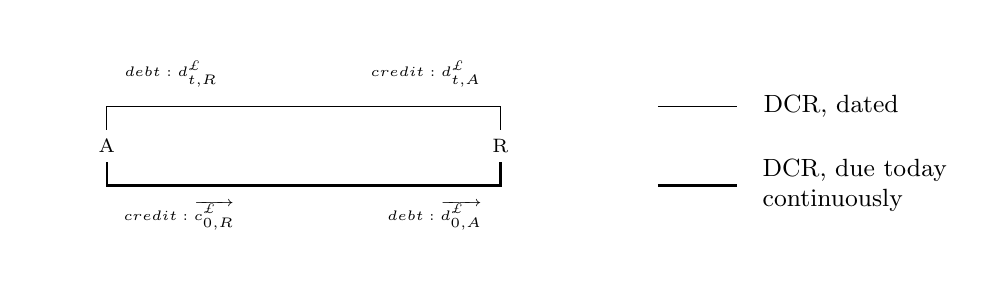
\begin{tikzpicture}
  \draw[help lines,white] (0,0) grid (12,3);
  % Left-hand side part of the Figure
  \node         (A)         at (1,1.5) {A};
  \node         (R)         at (6,1.5) {R};
  \draw[black]   (A.north) |- (4,2) -| (R.north);
  \draw[black,thick]   (A.south) |- (4,1) -| (R.south);
  \node at (3.5,2.4) {\textsuperscript{$debt: d^{\pounds}_{t,R}$ \hspace{.7in} $credit: d^{\pounds}_{t,A}$}};
  \node at (3.5,0.6) {\textsuperscript{$credit: \overrightarrow{c^{\pounds}_{0,R}}$ \hspace{.7in} $debt: \overrightarrow{d^{\pounds}_{0,A}}$}}; 
  % Labels
    \draw[black] (8,2) -- (9,2); \draw[black,thick] (8,1) -- (9,1);
    \node[black,align=left,font=\small] at (10.2,2) {DCR, dated};
    \node[black,align=left,font=\small] at (10.5,1) {DCR, due today\\continuously};
\end{tikzpicture}
\caption[Example of accommodation of the foreigner $A$ by the broker $R$ at the London money market]%
{Example of accommodation of the foreigner $A$ by the broker $R$ at the London money market\par\vspace{.05in}\par Source: narrative from \citep[p.~13]{keynes1971_1}, illustration by author.}
\label{fig:london_money_mkt}
\vspace{.2in}
\end{figure}

In other words, at the very moment when accomodation took place a foreigner had a British pound denomindated claim for immediate payment on a London banker (broker). Or, in the \citeauthor{innes1913}' terminology, a foreigner obtained a credit due today, immediately on that banker. Now, imagine that such accomodations of different foreigners took place at varying pace but continuously and numerously. Hence, on aggregate British banks had their balance sheets expanded upon accomodations by dated credits $c^{\pounds}_t$ on foreigners and by debts due today continuously $\overrightarrow{d^{\pounds}_0}$ owed to foreigners. As an mirror image the aggregate balance sheet of foreigners expanded by credits due today continuously $\overrightarrow{c^{\pounds}_0}$ on British banks and by dated debts $d^{\pounds}_t$ owned to British banks. And tenor $t$ of loan accomodations was within days, not months, due to short-term nature of the money market. And, surely, British banks were charging foreigners interest upfront (if discounting bills) or at maturity (if making loans). 

Hence, when Keynes was describing Great Britain as ``a country which is prediminantly a creditor" with respect to other countries he implicitly meant that a creditor country's banks hold dated credits against those other countries, or these are short loans loans falling due in certain number of days, and at the same time they owe to the same other counries debts due today continuously, or these are claims for immediate payment.

So, as \citeauthor{keynes1971_1} explained above, when the Bank of England feared a specie drain then it was thinking of such situaion when Britsh banks on a particular day would have inequality between credits they held on foreigners that were falling due today, $c^{\pounds}_0$, and debts due today continuously, $\overrightarrow{d^{\pounds}_0}$, which foreigners had ordered for conversion of these debts into specie: $c^{\pounds}_0 < \overrightarrow{d^{\pounds}_0}$. 

So Bank of England would attempt through raising the ``bank rate" (policy rate) to create such conditions, producing today and, if nessesary, each next day for the British banks a near match between their claims $c^{\pounds}_0$ on foreigners and debts $\overrightarrow{d^{\pounds}_0}$ owed to them \textit{and} who ordered them for specie conversion: $c^{\pounds}_0 = \overrightarrow{d^{\pounds}_0}$. Then, the British banks would apply the set-off principle,\index{Keynes, John M.!on set-off} meaning that foreigners have paid upon their due debts with British banks and no debts were left for specie conversion.

This exposition is not intended as showcase of gold-exchange standard operations. Instead, it is just an illustration that basic traces of the \acfp{dcr}--creation, re-use and set-off---were discussed by \citeauthor{keynes1971_1} albeit by utilizing a different vocabulary. His understanding of the monetary system operations evolved over his life time, becoming more sophisticated and wordly recognized. His \textit{A Treatise on Money} first published in \citeyear{keynes1930a} contained this observation as a preface to the main body of that volume: ``The ideas with which I have finished up are widely different from those with which I began."~\citep[p.~vi]{keynes1930a} His next observation from this work worth mentioning as an extention to the above mentioned discussion of the bank-rate policy made in the 1913 book \textit{Indian Currency and Finance}:

\begin{quote}
The gradual evolution of bank-rate policy under conditions, in London, peculiarly well adapted to it, coupled with a prodigious growth of Bank-Money, characterised British monetary developments [since the Bank Charter Ac of 1844] for the next seventy years. But, whilst the practical efficacy of bank-rate became not merely familiar but an article of faith and dogma, its precise \textit{modus operandi} and the varying results to be expected from its application in varying conditions \textit{were not clearly understood} -- and \textit{have not been clearly understood}, in my opinion, \textit{down to this day.}~\cite[p.~17, emphasis added]{keynes1930a}
\end{quote}

This critique as it appears was directed at the expectation that bank-rate policy could sustain the gold-exchange standard. Hence, the above-mentioned details with respect to banks of using set-off\index{Keynes, John M.!on set-off} or ``counterbalancing mutual claims of immediate payments" do remain useful. 

The first volume of the book \textit{A Treatise on Money} is divided into four main sections (called books), of which the first book called ``The Nature of Money" containts some analysis of payments especially with respect to state-money and bank-money. Emphasis on chartalism being in the driving seat on the concept of money is much more explicit than in \citeauthor{innes1913}. Thus, ``the State may then use its charttalist prerogative to declare that the debt itself is an acceptable discharge of a liability" \citep[p.~6]{keynes1930a}. However, \citeauthor{innes1913} provides more clarity on how debt itself discharges a liability -- it is done via conceptualization of \acfp{dcr} with debts and credits as well as debtors and creditors, and then via the set-off principle (see Section~\ref{sec:essential}, pp.~\pageref{sec:essential}-\pageref{sec:other_creditists}).

While describing creation of bank-money, \citeauthor{keynes1971_1} relied on the term that ``a bank creates claims against itself"~\citep[p.~23]{keynes1930a}. This is what was defined earlier in Figure~\ref{fig:london_money_mkt}, p.~\pageref{fig:london_money_mkt}, as debt due today coninuously, $\overrightarrow{d_0}$, denominated in some money of account. This is counterbalanced on the books of a bank by credit denominated in the same money of account.\footnote{For example, $\overrightarrow{d^{\$}_0}$ for U.S. dollar, $\overrightarrow{d^{\pounds}_0}$ for British pound, and $\overrightarrow{d^{\text{\rupee}}_0}$ for Indian rupee, $\overrightarrow{d^{\text{\textyen}}_0}$ for Japanese yen.} This credit could be dated or due today coninuously. If a bank's customer brings some form of state money or a check on another bank, then this is credit of the due-to-day-continuously type, $\overrightarrow{c_0}$. If a bank's customer borrows or sells some asset she holds, then this is dated credit, $c_t$. Hence, in this regard the works of \citeauthor{keynes1930a} and \citeauthor{innes1913} are rather similar.

In \textit{A Treatise on Money}, there is section three ``The Fundamental Equations" containing discussion of foreign transactions such as lending, borrowing and balances. The following definition of foreign lending is worth mentioning here:

\begin{quote}
By \textit{Foreign Lending}, on the other hand, we propose to mean what might, perhaps, be called the unfavourable balance of transactions on \textit{capital} account, i.e. the excess of the amount of our own money put at the disposal of foreigners through the net purchase by our nationals of investments situated abroad, over the corresponding amount expended by foreigners on the purchase of our investments situated at home.~\citep[pp.~131-132, emphasis original]{keynes1930a}
\end{quote}

The paragraph above was accompanied by a footnote: ``Loan Capital must be regarded as situated in the country of the debtor (whatever currency it may be expressed in)."~\citep[p.~132]{keynes1930a} 

This disseration considers such definition of foreign lending, with locality being predetemined or assigned to the country of a debtor and irrespective of denomination in money of account, as deviating from the concept of money as a \acf{dcr}. On this see Chapter~\ref{sec:payments}.

In his later writings on the post World War II reconstraction of the international economic and monetary systems, \citeauthor{keynes1980_25} developed a proposal on \acf{icu}. In it he referenced to the essential principle of banking,\index{Keynes, John M.!on principle of banking} which is not be found in \cite{innes1910,innes1913,innes1914}. It was formulated in the following way:

\begin{quote}
This principle [of banking] is the necessary equality of credits and debits, of assets and liabilities. If no credits can be removed outside the banking system but only transferred within it, the Bank \textit{itself} can never be in difficulty. It can with safety make what advances it wishes to any of its customers with the assurance that the proceeds can only be transferred to the bank account of another customer. Its problem is solely to see to it that its customers behave themselves and that the advances made to each of them are prudent and advisable from the point of view of its customers as a whole.~\citep[pp.~44-45]{keynes1980_25}
\end{quote}

\cite{wray1999} criticized \citeauthor{keynes1980_25}'s \ac{icu} proposal as having two problems. First one is that international monetary system cannot be designed as if trade were `goods against goods`. Second is that its banking analogy is confused. On one hand it is correctly asserts that elimination of convertibility of bancor, money of account in the \ac{icu}, into gold nullifies potential runs on the system. On the other hand, its assertion that balances in bancors might be ``employed to finance" further activity is ``flawed," because by endogenous money approach\index{Money!endogenous approach to} it is loans denominated in bancor create the reserve balances in bancor held by surplus nations \citep[p.~194-198, footnote 16]{wray1999}.\footnote{\cite{wray1999} was published in \cite{harvey1999}.}

%
% -------------- Joseph A. Schumpeter (1883-1946) ------------------------------+
%
\subsection{Joseph A. Schumpeter}\index{Schumpeter, Joseph A.}

\citeauthor{lakomski} observes in the \citeyear{lakomski} that ``Schumpeter belongs to a long tradition in economics that built a ``credit theory of money" (Schumpeter 1954) that can be associated with the likes of Henry Dunning Macleod (Skaggs 1997), A. Mitchell Innes (1914), and John Maynard Keynes (1930)"~\citep[p.~503]{lakomski}. In particular, Schumpeter ``recognized that banks do not carry out their activities in isolation, but are linked together and with a central bank, through a network of interbank debts and claims"~\citep[p.~502]{lakomski}. He held ``strong assumption that the money market is the ``headquarters" \dots or the ``heart" of the capitalist system"~\citep[p.~507]{lakomski}.\index{Schumpeter, Joseph A.!on money market}

That sticky description of the money market through the ``headquarters of capitalist system" metaphor is from \cite{schumpeter1934}. \citeauthor{minsky1986_} regarded this work and especially its chapter `Credit and Capital` as the highest point of \citeauthor{schumpeter1934}'s analysis of money and there was no advance beyond that level ever since by him~\citep[p.~112]{minsky1986_}.

A close read of \citep{schumpeter1934} and its chapter `Credit and Capital` that contains a section on the money market, pp.~123-127, reveals rather limited deail of how actually the money market operates. Consider the following extract:

\begin{quote}
\dots only one fundamental thing happens on the money market, to which everything else is accessory: on the demand side appear entrepreneurs and on the supply side producers of and dealers in purchasing power, viz. bankers, both with their staffs of agents and middlemen. \textit{What takes place is simply the exchange of present against future purchasing power.} In the daily price struggle between the two parties the fate of new combinations is decided.~\citep[p.~125, emphasis added]{schumpeter1934}
\end{quote}

The emphasized sentence from the quote above is too general and abstract, even though it somewhat resermbles the exchange depicted in Figure~\ref{fig:london_money_mkt}, p.~\pageref{fig:london_money_mkt}. 

In his major work on monetary theory \textit{Treatise on Money}, which was published first only 2008, \cite{schumpeter2014} described the monetary system and its operations in a more elaborate way than he did in the \citeyear{schumpeter1934} book \textit{The Theory of Economic Development}. Writing in 1986, \citeauthor{minsky1986_} recalled Paul Samuelson saying of this book: ``Schumpeter's response to the appearance of \textit{The General Theory} was to abandon his long-promised and in-process book on money"~\citep[p.~112]{minsky1986_}.

In \citep{schumpeter2014} one read chapters and sections with promising titles. Such as section ``How Payment Really Works" from chapter nine, and section ``The Money Market as Heart of the Capitalist Economy" from chapter twelve. However, the content in both of them brings very little of the analysis of how payments are done and how the money market operates.

The main substance of the operational details of the monetary system and the money market operations is in the chapters seven and eight, which are titled ``The Vehicles of the Social Accounting Process: The Banks and the Central Bank" and ``Bank-Mdeiated Money Creation," respectively. In there, \citeauthor{schumpeter2014} started with acknowledgment that ``bank-mediated payments predominate"~\citep[p.~156]{schumpeter2014}. While still his analysis of payments is in disadvantage if compared to \cite{innes1913}, \citeauthor{schumpeter2014} talked of bank operations in an extended detail, which allowed him to build an analytical thread from an individual bank that facilitated payments between own customers to a more complicated case of network of banks that was making payments between themselves on behalf of their customers. In the latter case, the money market and clearing house operations were brought into the foreground of his analysis. Consider the following quote, illusration of which would be rather close to one in Figure~\ref{fig:banks_clients_govt2}, p.~\pageref{fig:banks_clients_govt2}:

\begin{quote}
Rarely do banks work in disconnected fashion. From the very beginning
of the banking system and by the time of the Proven\c{c}al fair bankers, it was the
interbank exchange of claims or particularly organized interbank clearing that
was the heart of the banking system and the main girder of the edifice of bank
means of payment. Proliferation of the clearing function was also an important
motive behind the monopoly aspirations of the early city banks, as with, e.g.,
that of Barcelona. The clearinghouse enters the scene wherever there is a
multiplicity of banks, and once it is there, it shows a tendency to be a super-bank
and to provide help to individual banks in difficult situations, such as through the
issuance of clearinghouse certificates. In our picture, we let it be subsumed in
the central bank, to which indeed clearinghouses usually connect in terms of
organization.~\citep[p.~165]{schumpeter2014}
\end{quote}

The structure of the money system in the standard presentaion by \cite{schumpeter2014} is a bit more complex or uptodate than in Figure~\ref{fig:banks_clients_govt2} as it considers the central bank providing payment services to the government and banks, which have accounts wih it. The rest of the public, consisting of firms and households, is served by banks, i.e. not by the central bank. The latter in this simplified scheme is a bank of banks plus government, which however was not universially the case in practice. Thus, ``[t]he U.S. Reserve Banks have, e.g., no corporate customers, and few central banks maintain the smaller business customers to the degree that the Banque de France does"~\citep[p.~167]{schumpeter2014}. As a side note \citeauthor{schumpeter2014} elaborated a bit further on the possible extention of his analytical scheme: ``[i]t is also evident that the possibility of [corporate and other] customers' migrating to the central bank [from private commercial banks] can be an essential cog in the machine of any active central bank policy and, where it is missing, it is just this activity that, so to speak, is deprived of its spirs"~\citep[pp.~167-168]{schumpeter2014}. By saying this \citeauthor{schumpeter2014} was thinking of greater utility of direct \acfp{dcr} between the monetary authority and general public instead of a hierarchy of \acp{dcr}. In the latter case, there is a layer of \acp{dcr} between central bank and government plus banks, which then followed down below with a layer of \acp{dcr} between banks and general public (firms and households), see Figure~\ref{fig:schumpeter_scheme} on p.~\pageref{fig:schumpeter_scheme}.

The following quote of \cite{schumpeter2014} reveals his thinking of the impact of payments upon the balance sheets of different groups of the economic units in the society. He termed that impact as ``forcing funds onto customers". 

\begin{quote}
The power of the central bank over the reserve balances of banks (bankers' balances) is yet greater than the power of banks over customers' balances: to be specific, while banks
namely can cut credit to their customers but cannot easily force funds onto
customers who do not desire them, when the central bank buys securities, bank
reserves are increased whether the banks want this increase or not. How much or
how little this signifies will become clear to us later. At any rate, it means
\textit{additional liquidity} in the money market and elimination of the \textit{restraints} that can arise in business activity due to a shortage thereof. Conversely, the sale of
securities by the central bank signifies a contraction of reserve balances, a
``tightening" of credit offered by the banks and therefore, depending on
circumstances, a more or less palpable curb to business ardor.~\citep[p.~174, emphasis original]{schumpeter2014} 
\end{quote}

It must be recalled here that ``bankers' balances" and ``customers' balances" are conceptualized by this dissertaion as \acfp{dcr} of the due-today-continuously type. Bankers' balances are reserves for the central bank it is debts, $\overrightarrow{d_0}$, while for banks these are credits, $\overrightarrow{c_0}$. Customers' balances are debts the private banks, $\overrightarrow{d_0}$, and at the same time these credits, $\overrightarrow{c_0}$, for non-bank entities. Then, when \citeauthor{schumpeter2014} was saying``when the central bank buys securities, bank reserves are increased whether the banks want this increase or not," the most relevant part of this expression for us now is when banks did not want that increase in reserves. The central bank forced funds onto banks by buying securities from non-bank entities. This can be illusrated, using Figure~\ref{fig:schumpeter_scheme}, via an example of cenral bank $CB$ buying securities from individual $C$, who is customer of bank $R_2$. Upon the purchase of these securities of a certain money volume, the payment by buyer $CB$ to seller $C$ results in an increase in two \acfp{dcr}: (1) between central bank and bank $R_2$, and (2) between bank $R_2$ and individual $C$. In the \citeauthor{schumpeter2014} the central bank forced funds onto private bank. Hence, he concluded that central bank is able to do it with its customers which are private banks, while the latter cannot do it ``easily" with their own customers. 

It might be argued that banks customers would welcome bank ``forcing funds onto" them if these are without a forced counter claim of dated debt. In other words, it is a situation, when a customer's credit on her bank has increased, $\overrightarrow{c_0}$, and customer's debt owed to the same bank due in some future time, $d_t$, has not, meaning her net worh or equity has been boosted. This is a valid counter argument, while it alludes to a situation which is out the main business arsenal of the for-profit undertakings such as banks. 

Continuing the discussion of the quote above another point must be made. If one adds to the \citeauthor{schumpeter2014}'s scheme the fact that some smaller banks opt to have accounts with larger commercial banks and not having a direct account with the central bank, then the above claim made by \citeauthor{schumpeter2014} requires modification. Banks maintain with each other \acfp{dcr} of the due-today-continuously type. These are called correspondent accounts and thier function is identical to the checking accounts or current accounts or demand accounts that banks open and maintain with their non-bank customers such as government, firms and private individuals. In the U.S., the same type of the account a member bank has with the Federal Reserve Bank is referred to as reserves account. Behind all these names lies one function of such an account and it representing a \acf{dcr} due today continuously: a debtor bank is on the debt side of this relationship and its account balance is marked as $\overrightarrow{d_0}$, while a creditor bank is on the credit side of it and has a balance on this account marked $\overrightarrow{d_0}$. So, both balances $\overrightarrow{d_0}$ and $\overrightarrow{c_0}$ idenical in terms of (a) money of account, (b) size expressed in some digits, and (c) tenor, which is today or $t=0$ all the time or continuously.

In Figure~\ref{fig:schumpeter_scheme}, there is bank $R_3$ that has no direct correspondent account with the central bank and instead it has such an account with bank $R_1$. Hence, bank $R_3$ is a customer of bank $R_1$ on quite the same principles as other customers: individuals $A$ and $B$. It has its own customers $E$ and $F$. Then, consider an example of central bank purchasing securities from $F$. Upon the purchase of these securities of a certain money volume, the payment by buyer $CB$ to seller $F$ results in an increase in three \acfp{dcr}: (1) between central bank and bank $R_1$, (2) between bank $R_1$ and bank $R_3$, and (3) between bank $R_3$ and individual $F$. 

This examples serves as an extention to the \citeauthor{schumpeter2014} that banks, unlike the central bank, cannot ``force funds onto their customers" easily. If a bank customer is another, correspondent bank then such development takes place. The main feature is that an economic entity, which is not a central bank itself, that maintains \acfp{dcr} due today continuously, $\overrightarrow{d_0}$, being on the debt side with its customers is able to do it only if it is able to maintain the same type of \acp{dcr} being on the credit side as a customer of another such entity or the central bank. Hence, this is a definitive characteristic of a banker that once it managed itself into such a position with respect to own debts owed to its customers then it is in a business of acommodating own customers not only as payers, initiators of payments, but quite importantly as payees, reciepeints of payments.

It implies, too, that in the \citeauthor{schumpeter2014}'s analysis the term liquidity is associated with changes of \acfp{dcr} due today continuously between certain entities of the economy. This is especially evident from his discussion of the impcat the government's spending and taxing operations have with respect to banker's balances with the central bank. 

\begin{quote}
No matter what the central banks otherwise are \dots for us
they are simply \textit{banks' banks}, everything else is secondary. However, at the same time we wish in every region to allow them to be the government's bank, into which taxes are deposited and which make the state administration's
disbursements, and which thus conduct the public accounts, which in England is
the case at its purest. We do this because in this case, tax payments and
government spending, beyond their usual meaning for the money process, are
accorded yet another special theoretical interest that they would otherwise lack
and which deserves to be highlighted. That is to say, government expenditure
which is effected by a check drawn on funds of the state administration at the
central bank, increases the reserve funds of the bank of the recipient of the
payment, and thus facilitates credit expansion just like a gold inflow.
Tax collection has the opposite effect, so that in this case a tightening or loosening
effect on the money market proceeds from the financial management of the
state, which comes on top of the influence that financial management already
exerts in all cases.~\citep[pp.~166-167, emphasis original]{schumpeter2014} 
\end{quote}

We can extend this discussion into the one based upon a more general term of \acf{dcr} due today continuously. Assume priorily that central bank and government have at the moment a \acf{dcr} of enough size or balance. Then, when government $G$ makes a payment in favor of individual $C$, as they are shown in Figure~\ref{fig:schumpeter_scheme}, then such a payment produces (a) decrease in the \ac{dcr} between $CB$ and $G$, and (b) an increase in two \acp{dcr}: (1) between $CB$ and bank $R_2$, and (2) between $R_2$ and individual $C$, the reciepient of the government payment. If, instead, the government $G$ makes a payment in favor of individual $F$ then such a payment results in an increase in three \acp{dcr}: (1) between $CB$ and bank $R_1$, (2) between $R_1$ and bank $R_3$, and (3) between bank $R_3$ and individual $F$, the reciepient. The opposite changes of \acp{dcr} will take place, when individuals $C$ and $F$ pay taxes in favor of government. 

\citeauthor{schumpeter2014} never used the concepts this dissertation proposes. While his money system scheme is typical for the modern-day structure, however, it needs extention to account for more complex domestic relationships and then their further spread into cross-border realm. More so as \citeauthor{schumpeter2014} opted ``not \dots to complicate our depiction by introducing international credit relations"~\citep[p.~184]{schumpeter2014}.

There is critique of \citeauthor{schumpeter2014} work such as by \cite{earley1994}, which also relied on the analysis of the original version of the manuscript \textit{Das Wesen des Geldes}, which much later become known in English translaion as \textit{Treatise on Money}. It appears that \citeauthor{earley1994} writing in \citeyear{earley1994} had access to the German manuscript via his doctorate student \citeauthor{reclam1984}, a native German himself. While as a book \textit{Das Wesen des Geldes} was published only in 2008. Its translation in English appeared only in 2014. Thirty year prior, \citeauthor{reclam1984} wrote his disseration work titled \textit{J. A. Schumpeter's 'Credit' Theory of Money} and had \citeauthor{earley1994} as his chair of the advasory committee. At the very beginning \citeauthor{reclam1984} had an idea of translating the German manuscript \textit{Das Wesen des Geldes} into English and publish it as a book. However, he and \citeauthor{earley1994} consulted with \citeauthor{schumpeter2014}'s scholars on this project. The latter concluded that it had nothing new if compared to \citeauthor{schumpeter1939_1}'s book \textit{Business Cycles}. \citeauthor{reclam1984} decided to use the manuscript as basis for his dissertation work \citep{reclam1984}.

So, main point of critique by \cite{earley1994} is that Schumpeter never departed from the Quesnay-Walras concept\index{Quesnay-Walras concept} of a ``circular flow" of economic life. That concept explains money as being circulation throught the economy as blood circulates through the human body. ``This vision became part of Schumpeter's own, and it stayed with him to the end"~\cite[p.~344]{earley1994}. Even though Schumpeter was actively writing on the credit theory of money, in his thinking money and credit were circulaing around the economy as a thing. Moreover, his conception of money of account is quite different from that of \citeauthor{keynes1930a} and \citeauthor{innes1913}.

For Schumpeter money of account is a unit of account that one can count and hence there are many units of account, which are subject to distribution and redistribution via hand to hand payments, if units are tokens, or bank-mediated payments, if units are debts and credits. It means that if a bank account of a person had a balance of 5 Mexican pesos, then it contained 5 units in terms of Mexican pesos. Likewise, if another person had in her pocket 5 Mexican pesos in coins. For Keynes money of account is a title---such as dollar or peso---being decided by the state authority and it is used to express, or denominate, debts, prices and contracts. Hence, there is one money of account per community or society being organized through the power of state. Example, the US dollar is money of account in the United States, while Mexican peso is moeny of account in Mexico, and so on. This is an approach held by \citeauthor{innes}. If society has several money of account than it is a sign of less harmony. That is why some economists proclaim ``one government, one money" \citep{goodhart2017} or ``one nation, one currency" \citep[pp.~41-42]{wray2012}. Also, \citeauthor{wray2009} recognizes that Schumpeter's ``vision of markets was much more orthodox" \citep[p.~810]{wray2009}.

Lastly, the following observation made by Schumpeter in his \textit{Treatise on Money} has analytical value, especially as next subsection turns to the analytical framework developed by \citeauthor{minsky1986}:

\begin{quote}
Banks also do other things than those that one thinks of with the words
money and credit transactions. Some conduct e.g. merchandise departments \dots. We intend to disregard these as well as ancillary businesses such as
safe deposit box rental; but currency metal trading, investments and divestments \dots and securities issues (not securities trading on behalf of others) are partly so common and partly, in some countries, so important for understanding the functioning of the monetary
mechanism and so inseparable from the lending business, that we cannot (or can
only in a specific case), exclude them from our depiction. We cannot even
exclude them where the banks do not ``go public'' and where they do not, as they
do in Germany, play a direct role in industry, which is contrary to their nature
and restrictive to their functioning. The basic outline of the matter is only clear when we imagine that the entire payment and credit system of transactions centers in the banks.~\citep[p.~154]{schumpeter2014}
\end{quote}

\begin{figure}[!ht]
\vspace{.0in}
\captionsetup{width=1\linewidth,labelfont=bf}
  \centering
  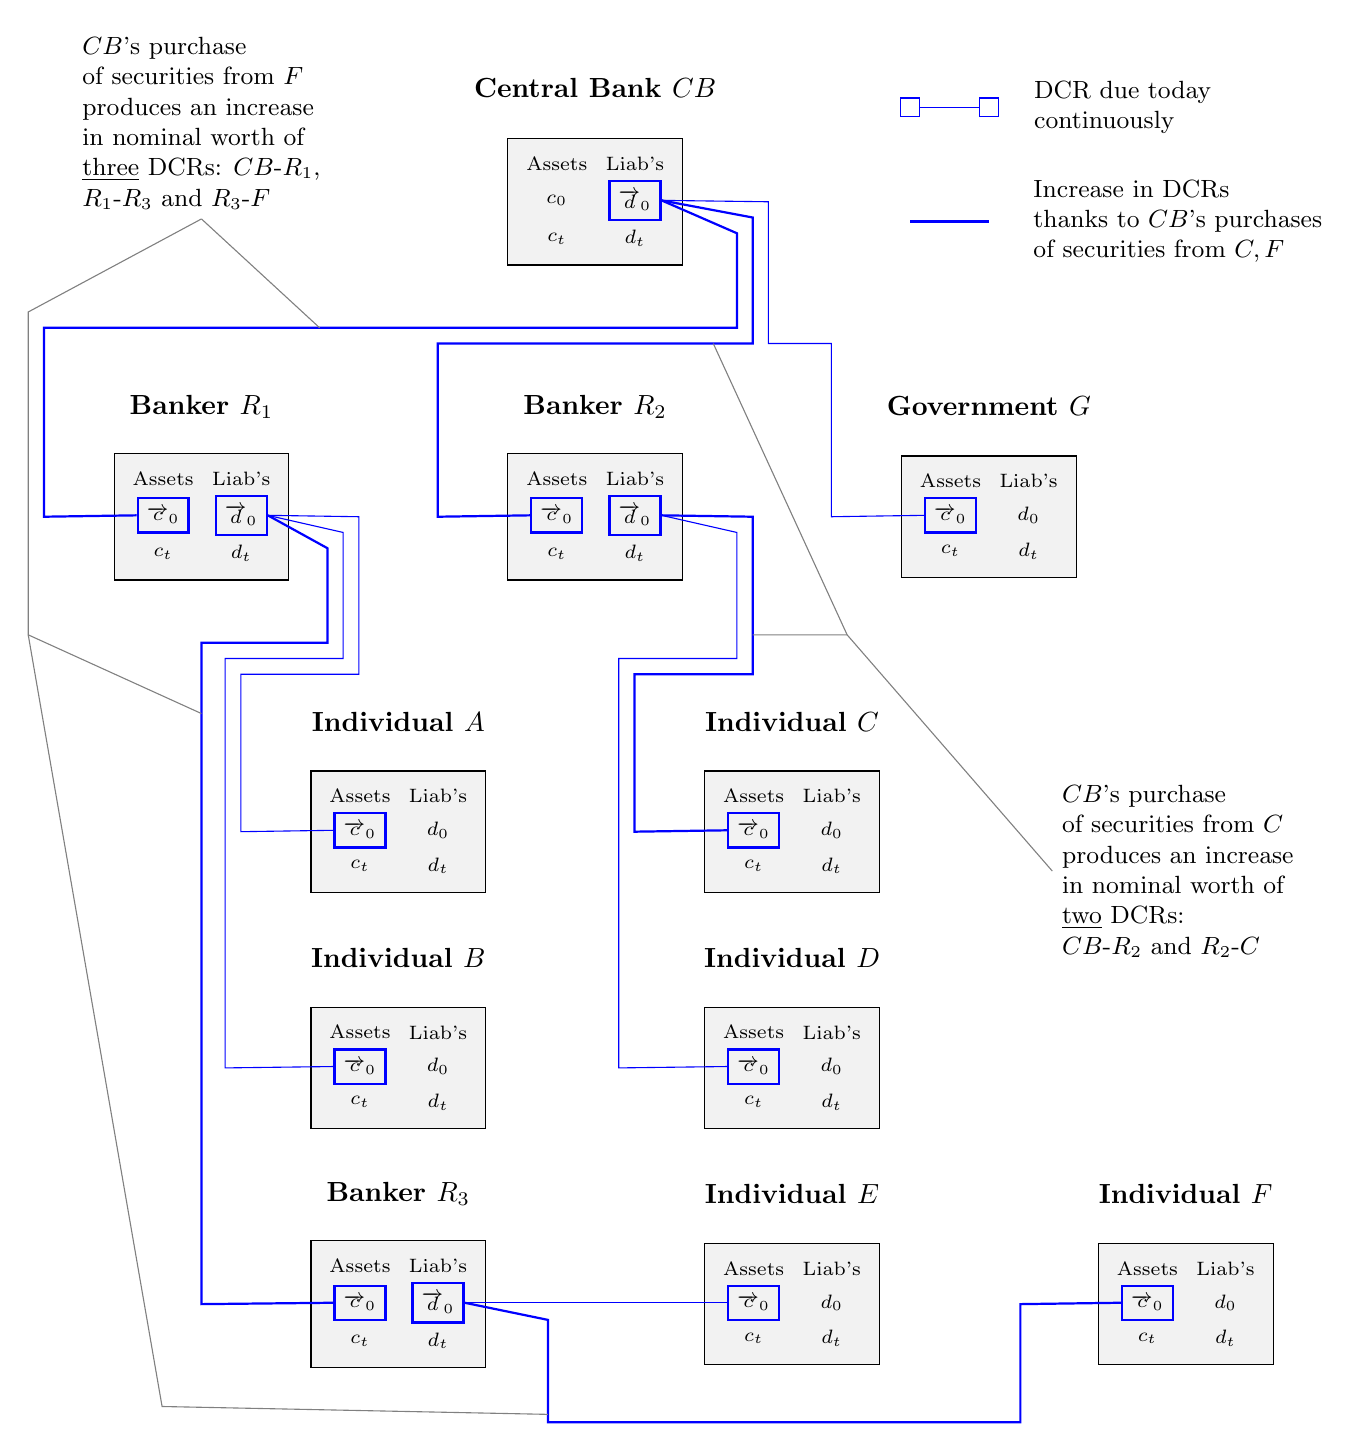
\begin{tikzpicture}
  \draw[help lines,white] (0,0) grid (16,14);  
        % BS of govt (issuer of "lawful money") -----------------------------
        \node [matrix,fill=gray!10,draw=black,thin] (cb) at (7,13)
          {
            \node {Assets}; & \node {Liab's}; \\
            \node (CB_c0) {$c_0$}; & \node[rectangle,draw=blue,thick] (CB_d0)  {$\overrightarrow{d}_0$}; \\
            \node {$c_t$}; & \node {$d_t$}; \\
          };
          \draw (cb)++(0,1.45) node[font=\bf]{Central Bank $CB$}; 
        % BS of banker R1 ---------------------------------------------------
          \node [matrix,fill=gray!10,draw=black,thin] (r1) at (2,9)
          {
            \node {Assets}; & \node {Liab's}; \\
            \node[rectangle,draw=blue,thick] (R1_c0) {$\overrightarrow{c}_0$}; & \node[rectangle,draw=blue,thick] (R1_d0)  {$\overrightarrow{d}_0$}; \\
            \node {$c_t$}; & \node {$d_t$}; \\
          };
          \draw (r1)++(0,1.4) node[font=\bf]{Banker $R_1$}; 
          \node [matrix,fill=gray!10,draw=black,thin] (r2) at (7,9)
          {
            \node {Assets}; & \node {Liab's}; \\
            \node[rectangle,draw=blue,thick] (R2_c0) {$\overrightarrow{c}_0$}; & \node[rectangle,draw=blue,thick] (R2_d0)  {$\overrightarrow{d}_0$}; \\
            \node {$c_t$}; & \node {$d_t$}; \\
          };
          \draw (r2)++(0,1.4) node[font=\bf]{Banker $R_2$};
          \node [matrix,fill=gray!10,draw=black,thin] (g) at (12,9)
          {
            \node {Assets}; & \node {Liab's}; \\
            \node[rectangle,draw=blue,thick] (G_c0) {$\overrightarrow{c}_0$}; & \node (G_d0)  {$d_0$}; \\
            \node {$c_t$}; & \node {$d_t$}; \\
          };
          \draw (g)++(0,1.4) node[font=\bf]{Government $G$};
        % BS of private individuals -----------------------------------------
          \node [matrix,fill=gray!10,draw=black,thin] (a) at (4.5,5)
          {
            \node {Assets}; & \node {Liab's}; \\
            \node[rectangle,draw=blue,thick] (A_c0) {$\overrightarrow{c}_0$}; & \node {$d_0$}; \\
            \node {$c_t$}; & \node {$d_t$}; \\
          };
          \draw (a)++(0,1.4) node[font=\bf]{Individual $A$};
          \node [matrix,fill=gray!10,draw=black,thin] (b) at (4.5,2)
          {
            \node {Assets}; & \node {Liab's}; \\
            \node[rectangle,draw=blue,thick] (B_c0) {$\overrightarrow{c}_0$}; & \node {$d_0$}; \\
            \node {$c_t$}; & \node {$d_t$}; \\
          };
          \draw (b)++(0,1.4) node[font=\bf]{Individual $B$};
          \node [matrix,fill=gray!10,draw=black,thin] (c) at (9.5,5)
          {
            \node {Assets}; & \node {Liab's}; \\
            \node[rectangle,draw=blue,thick] (C_c0) {$\overrightarrow{c}_0$}; & \node {$d_0$}; \\
            \node {$c_t$}; & \node {$d_t$}; \\
          };
          \draw (c)++(0,1.4) node[font=\bf]{Individual $C$};
          \node [matrix,fill=gray!10,draw=black,thin] (d) at (9.5,2)
          {
            \node {Assets}; & \node {Liab's}; \\
            \node[rectangle,draw=blue,thick] (D_c0) {$\overrightarrow{c}_0$}; & \node {$d_0$}; \\
            \node {$c_t$}; & \node {$d_t$}; \\
          };
          \draw (d)++(0,1.4) node[font=\bf]{Individual $D$};
          \node [matrix,fill=gray!10,draw=black,thin] (r3) at (4.5,-1)
          {
            \node {Assets}; & \node {Liab's}; \\
            \node[rectangle,draw=blue,thick] (R3_c0) {$\overrightarrow{c}_0$}; & \node[rectangle,draw=blue,thick] (R3_d0)  {$\overrightarrow{d}_0$}; \\
            \node {$c_t$}; & \node {$d_t$}; \\
          };
          \draw (r3)++(0,1.4) node[font=\bf]{Banker $R_3$};
          \node [matrix,fill=gray!10,draw=black,thin] (e) at (9.5,-1)
          {
            \node {Assets}; & \node {Liab's}; \\
            \node[rectangle,draw=blue,thick] (E_c0) {$\overrightarrow{c}_0$}; & \node {$d_0$}; \\
            \node {$c_t$}; & \node {$d_t$}; \\
          };
          \draw (e)++(0,1.4) node[font=\bf]{Individual $E$};
          \node [matrix,fill=gray!10,draw=black,thin] (f) at (14.5,-1)
          {
            \node {Assets}; & \node {Liab's}; \\
            \node[rectangle,draw=blue,thick] (F_c0) {$\overrightarrow{c}_0$}; & \node {$d_0$}; \\
            \node {$c_t$}; & \node {$d_t$}; \\
          };
          \draw (f)++(0,1.4) node[font=\bf]{Individual $F$};
          % Debt-credit pairs due today continiously: G vs R1,R2,R3 ------------
          \draw[blue,thick] (R1_c0.west) -- (0,9) -- (0,11.4) -- 
                (8.8,11.4) -- (8.8,12.6) -- (CB_d0.east); %\draw[blue,thick] (0.4,10.6)--(0.4,11.2);
          \draw[blue,thick] (R2_c0.west) -- (5,9) -- (5,11.2) -- 
                (9,11.2) -- (9,12.8) -- (CB_d0.east); %\draw[blue,thick] (5.4,10.4)--(5.4,11.2);
          \draw[blue,thin] (G_c0.west) -- (10,9) -- (10,11.2) -- (9.2,11.2) -- (9.2,13) -- (CB_d0.east);
          \draw[blue,thick] (R3_c0.west) -- (2,-1) -- (2,7.4) -- 
                (3.6,7.4) -- (3.6,8.6) --  (R1_d0.east); %\draw[blue,thick] (5.4,10.4)--(5.4,11.2);
          \draw[blue,thin] (A_c0.west) -- (2.5,5) -- (2.5,7) -- (4,7) -- (4,9) -- (R1_d0.east);
          \draw[blue,thin] (B_c0.west) -- (2.3,2) -- (2.3,7.2) -- (3.8,7.2) -- (3.8,8.8) -- (R1_d0.east);
          \draw[blue,thick] (C_c0.west) -- (7.5,5) -- (7.5,7) -- (9,7) -- (9,9) -- (R2_d0.east);
          \draw[blue,thin] (D_c0.west) -- (7.3,2) -- (7.3,7.2) -- (8.8,7.2) -- (8.8,8.8) -- (R2_d0.east);
          \draw[blue,thin] (R3_d0.east) -- (E_c0.west);
          \draw[blue,thick] (R3_d0.east) -- (6.4,-1.2) -- (6.4,-2.5) -- (12.4,-2.5) -- (12.4,-1) -- (F_c0.west);
          % Labels
          \draw[blue] (11,14.2) node(a)[draw] {} (12,14.2) node(b)[draw] {};
          \draw[blue] (a) -- (b);
          \node[black,font=\small,align=left] at (13.7,14.2) {DCR due today\\continuously};
          \draw[blue,thick] (11,12.75) -- (12,12.75);
          \node[black,font=\small,align=left] at (14.4,12.75) {Increase in DCRs\\thanks to $CB$'s purchases\\of securities from $C,F$};
          % Text labels
          \node[black,font=\small,align=left] (txt) at (14.4,4.5) {$CB$'s purchase\\of securities from $C$\\produces an increase\\in nominal worth of\\\underline{two} DCRs:\\$CB$-$R_2$ and $R_2$-$C$}; \draw[gray] (txt.west) -- (10.2,7.5) -- (9,7.5);
          \draw[gray] (10.2,7.5) -- (8.5,11.2);
          \node[black,font=\small,align=left] (txt) at (2,14) {$CB$'s purchase\\of securities from $F$\\produces an increase\\in nominal worth of\\\underline{three} DCRs: $CB$-$R_1$,\\$R_1$-$R_3$ and $R_3$-$F$}; \draw[gray] (txt.south) -- (3.5,11.4);
          \draw[gray] (txt.south) -- (-.2,11.6) -- (-.2,7.5) -- (2,6.5);
          \draw[gray] (-.2,7.5) -- (1.5,-2.3) -- (6.4,-2.4);
  \end{tikzpicture}
 \caption[Debt-credit pairs due today continuously: government, central bank, banks and general public]%
  {Debt-credit pairs due today continuously: government, central bank, banks and general public, which are denominated in the single money of account such as dollar (\$), between government ($G$), cenral bank ($CB$), banks ($R_1, R_2, R_3$) and general public ($A,B,C,D,E,F$).\par\vspace{.05in}Note: (a) the dollar (\$) as money of account is not shown explicitly on this Figure, however, it is assumed to be used to denominate all debts and credits; (b) $t$ is tenor of debts and credits.}
  \label{fig:schumpeter_scheme}
  \vspace{.0in}
\end{figure}

%
% -------------- Hyman P. Minsky (1919-1996) -----------------------------------+
%
\subsection{Hyman P. Minsky}\index{Minsky, Hyman P.}

\citeauthor{minsky1992} had \citeauthor{schumpeter2014} as his Ph.D. advisor at Harvard University, who among other several economists influenced him to a considerable extent \citep{toporowski2008,wray2015_}. He picked up from \citeauthor{schumpeter2014} endoegenous money approach, evolutionary processes and innovations driven by profit-seeking enterprenuers. Hence, the following credit given a short paper written in \citeyear{minsky1992}:

\begin{quote}
Schumpeter brought to the analysis of a monetary producion economy the sense of the economy as an evolving institutional sructure. \dots The Schumpeter-Keynes vision of the economy as evolving under the stimulus of perceived profit possibilities remain valid.~\citep[p.~113]{minsky1992}
\end{quote}

Minsky extended the evolutionary processes and proft-seeking motives by enterprenuers into the sphere of finance, where innovations of financiers might lead not to the furthering of capital development of the economy and its society, a progressive process, but to increased financial instability. This is what Minsly termed as ``retrograde" process of evolution. 

It appears that Minsky followed Schumpeter by adopting the abstraction of ``circular flow" stating that ``[m]oney, in effect, goes around an income circuit"~\citep[p.~223]{minsky1986}.
One of his most used terms is of ``cash flow(s)," which at closer inspection mean payment(s). Thus:

\begin{quote}
\dots the economy we live our lives in is a capitalist economy that invests. In such an economy, the financing of investment and of ownership of the stock of capital assets leads to commitments to make money \textit{payments}, that is, to contractual cash flows.~\citep[pp.~157-158, emphasis added]{minsky1986}\par
\end{quote}

Indeed, analytically the framework that \citeauthor{minsky1986} applies in his writings is based upon the logic of payments, which do affect the balance sheets of different economic entities from government to central bank and from private banks to firms and individuals. And it fits well into what was discussed above. The following analysis in based upon Chapters 9 and 10 from \cite{minsky1986}.

As a very early point of the analysis \citeauthor{minsky1986} imagines an economic system this way: ``[t]he \textit{payment} commitments come due and are discharged as the economy moves through time"~\citep[p.~219, emphasis added]{minsky1986}. The payment commitments are recognized as contractual relationships between counter parties which make transactions. Hence, commitment to make payment is the same concept as one used above: \acf{dcr} between one entity, which is debtor, and another, which is creditor, and where the debtor must make payment on due date and, if the debtor failed to do so, the creditor has right to sue for non-payment.

In the following two quotes \cite{minsky1986} makes effectively similar statements as by \cite{innes1913} with respect to bank money and government's money, however using slightly different terminology:

\begin{quote}
Bank loans, while ostensibly money-today for money-later contracts, are really an exchange of debits from a bank's books today for credits to a bank's books later.'\par In an economy where government debt is a major asset on the books of the deposit-issuing banks, the fact that taxes need to be paid gives value to the money of the economy. The virtue of a balanced budget and a surplus insofar as the commodity value (purchasing power) of money is concerned is that the need to pay taxes means that people work and produce in order to get that in which taxes can be paid.~\citep[p.~258, including footnote 10]{minsky1986}
\end{quote}

In the first paragraph of the quote above, the definition of the bank loan as ``money-today for money-later contract" implies that two sides, the banker and the borrower, agreed to to have against each other the following liabilities: (1) ``money-today" is liability of the banker towards the borrower, while (2) ``money-later" is liability of the borrower towards the banker. And on the book, balance sheet, of the banker this contract leaves, once the borrower's payment is made in favor of a third party, a record of ``debits," which reflect the size of the loan by which the account of bank's credit on borrower increased. Here it must be recalled the accounting principles and terminilogy: when debits are recorded against the account, which seats in the asset side of the balance sheet of the banker, then it means that numerical balance of this account is marked \textit{up} by the size of debits; conversely, when credits are recorded against this account, then it means that it is marked \textit{down} by the size of credits. While ``credits" part must take place later at the end of the loan agreement. This description is identtical to the illustration of bank loan made above, see Figure~\ref{fig:bank_mk_loan}, p.~\pageref{fig:bank_mk_loan}.

As for the second paragraph, it is enough to say that its logic is the same as explained by \citeauthor{innes1913}' quote on p.~\pageref{fig:debt_credit_rel2}, see as well Figure~\ref{fig:debt_credit_rel2} on the same page.

Then, the next building bloc of Minsky's analytical framework is expressed in the following observation, which is rather a recommendation about an analytical angle:

\begin{quote}
To analyze how financial commitments affect the economy it is necessary to look at economic units in terms of their cash flows. The cashflow approach looks at all units---be they households, corporations, state and municipal governments, or even national governments---as if they were banks.\par Traditional banking literature emphasized the need for bankers to be liquid and solvent \dots the cash flows from business sales would lead to payments to banks; these payments would guarantee bank liquidity and solvency. In a similar way ordinary business needs to be liquid and solvent; this means that the payment commitments on debts must lie within bounds given by realized and expected cash flows.~\citep[p.~221]{minsky1986}
\end{quote}

Hence, every economic unit, or entity, makes payments as payer and is recepient of payments as payee on a regular basis. And the concept of liquidity and solvency appears in the Minsky's aparathus. It somewhat similar to the solvency Equations \ref{eq:solv_rule} and \ref{eq:solv_rule_banker} mentioned above on p.~\pageref{eq:solv_rule} and p.~\pageref{eq:solv_rule_banker}. However, conceptually the Minsky's thinking on liquidity and solvency is more complex and more structured approach then in the writings by \citeauthor{innes1913}. While \citeauthor{minsky1986} starts with individual entity, his point of desination is definitely and unmistakenly about the entire economic system \citep{bezemer2021}. Also, quite importantly \citeauthor{minsky1986} elevates to prime spot the issue of payment (``cash flow") origin: whether it is originated as earned funds thanks to sale of own goods or services or it is originated from borrowing funds.

In the Minsky's analytical framework there is a taxonomy of payments (``cash flows") by their origin: (i) income, (ii) balance sheet, and (iii) portfolio. The second type---the balance sheet type of payments---has own classification by tenor or maturity of the counter balancing item in the unit's balance sheet: (a) dated, (b) demand, and (c) contingent. Out of these three, the dated balance sheet payments are of two types in terms of an financial instrument (financial contract) employed: (1) the discounted note, and (2) the bond. See \citep[pp.~223-227]{minsky1986}. 

The typology in terms of \textit{origin} is explained this way. The first type of income payments relates to those payments, where an economic unit acting both as payee and payer experiences such impact on its balance sheet so that the change in the assets is counter balanced by change in own net worth or equity. In other words, such payments do not produce change in liabilities. The second type is of payments that result in change of liabilities, which are future payment commitments differing between themselves by tenor. The third type is about payments producing a change in the unit's assets.

The typology of the balance sheet payments in terms of \textit{tenor} is elaborated the following way. 

The first type of \textit{dated} payments means that a unit is to make payment or a series of payments in the future. If a date balance sheet payment is contracted as discounted note, then it has one future payment of a predetermined size. Another type of dated balance sheet payments is a financial contract of the bond. The latter means that there is a series of future payments of, again, predetermined size, not just one, and these are spread out in time. An extreme case of a bond is consol, which has future payments lasting forever or into perpertuity. The normal case of the bond is that payment commitments are over a certatin period of time: over one year or over five years and so on. This bond itself might be contracted in a number of ways such as a bullet bond or an amortization bond. Both make regular payments (called coupon payments) at a fixed rate relative to principal, the nominal value of the bond. The difference between them is how the payment of the principal is contracted. The bullet bond is a commitment to make payment of the principal at the very end of the bond's life, i.e. 100\% of principal is paid upon maturity of the bond. The amortizaion bond is a commitment to make payment of the principal at predetermined schedule, not exclusively on the maturity date, such as 25\% of principal to be paid alongside with coupon payments during every last four payments committed by this bond. In extreme case, an ammortization bond spreads out the payment of the principal over the entire life of the bond. In this case, both coupon payments and partial principal payments produce equal payments through maturity of the bond -- in other words, such a bond turns into a type of financial contract referred to as stable annuity.\footnote{Stable annuity type means a financial contract lasting a certain period of time and payment commitments upon it are of stable or equal size.} For example, ``[a]n automobile loan contract or home morgage reguires monthly payments of stipulated amount"~\citep[p.~224]{minsky1986}. 

Minsky's concept of dated payments (``cash flows') is in close equivalence with what was termed above as dated \acf{dcr}, $d_t$ and $c_t$ with $t geq 0$ standing for number of days from today till the maturity, expriration or end of tenor. Minsky's payment is frequently substituted with payment commitment, which now is in straight equivalence with \ac{dcr} because both imply the same thing.  

The second type of balance sheet payments is \textit{demand} contracts, upon which the payment is made on demand from the counter party. In Minsky's own words: 

\begin{quote}
\dots we have financial contracts of \textit{indeterminate duration}, which are phrased as demand contracts. The most important demand contracts are deposits at commercial banks and other depository financial institutions, such as savings banks. Of particular importance are the deposits subject to check, which are readily spent on current activity, moved from one bank to another, or exchanged for other assets. Such deposits are \textit{the principal form of money in our economy}.~\citep[p.~225, emphasis added]{minsky1986}.
\end{quote}

Even though, these contracts have ``indeterminate duration"\index{Duration!measure of time} by design, potentially lasting forever or into perpetuity, but these are not the bonds of the consol type mentioned above. Minsky's used the word ``duration" to allude to the tenor feature of this type of contract: in a sense that payment commitment might be triggered at will of the counter party or any time the latter desires. So, the tenor is indetermined, it might be today or tomorrow or some on other futture day. However, this dissertation relies on the word ``duration" in other sense as ``a measure of interest-rate risk" \citep{fabozzi2022}. The difference between two terms---duration as a measure of time\index{Duration!measure of time} and duration as a measure of interest-rate risk\index{Duration!measure of interest-rate risk}---was discovered in the practice of the financial industry only in the 1990s, as explained in \citep[p.~9]{fabozzi2022}. The demand contracts by design are zero-duration conracts -- it means their present value has zero interest-rate risk or, if said differently, when market inerest rate changes their value does \textit{not} change. This is in a sriking difference with consol bonds or any other dated contracts on which payment by design is spread out over time. And these contracts have duration greater than zero and, hence, their present value does change when market interest rate change in an opposite way. 

For example, if market inerest rate increases then an existing bond with no embedded options and remaining time to maturity of 10 years will experience an immediate drop in market price, its present value, and the difference between current price and previous price corresponds approximattely to duration in percentage terms. So, for such a bond, depending on predetermined coupon rate and ammortization of the principal, it must be somewhat lower than 10. For example, if exact duraion of the above-mentioned bond is 8, then an increase in the market interest rate by one percentage point, from 3.5\% to 4.5\%, results in about 8\% drop of the bond's price. And vise versa when interest rate decreases by 1\%~\citep[see][p.~198, formula 9-2]{fabozzi2005}.\index{Duration!measure of interest-rate risk}

To conclude, Minsky's observation of the existance of the special contracts of the demand type must be extended by saying that by design they have determined duration of zero, meaning their nominal value insensitive to the makret interest rate change. And, indeed, these contracts are ``the principal form of money in our economy." Minsky's demand contract is an equivalent to the concept of \acf{dcr} due today continously---with opposite positions $\overrightarrow{d_{0}}$ and $\overrightarrow{c_{0}}$ on its two sides---which was discussed above. Hereinfater these concepts are considered idenical and the latter one is to be used frequently.

Then, the third type of balance sheet payments is another special type after the demand one that is called conditional or \textit{contingent}. These are contracts upon which there is an endorsement from a third party such as governemnt or some state agency. These contracts are various insuarence contracts, conditional to certain events that migh be triggered or not. Also a common shareholder cotnract belongs to this category:

\begin{quote}
\dots the common stock of corporations embody contingent claims \dots The contingent claim of the common stockholder, for example, is to a proportional share of earnings, if they exist and are distributed, or to a proportional share of the value of the company if sold or liquidated. The value of common shares therefore is intimately related to the expected course of the cash flows that will remain with a firm after payment of contractual commitments on debts.~\citep[p.~226, emphasis added]{minsky1986}.
\end{quote}

So a for-profit undertaking has contingency debts which in sizable extent relate to its shareholders, whether it is a single shareholder or many shareholders. Their claims on such a business are residual claim to the value of this business that remains after payment upon all other types of debt (demand and dated). In this disseration, these are labelled as $\widetilde{d}$.

Sizable part of the for-profit undertakings derive their income payments by producing and then selling goods to the customers or services of non-financial character. These firms rely on their positons in capital assets. These are items that belong to the assets side of the balance sheets of these firms. Hence, they are groupped alongside with as credit positions(dated and demand) within \acfp{dcr} with respective counter parties. Since, value of capital assets is above zero if they are expected to yield future quasi-rents as income payments, then these are contingent credits. These quasi-rents are not dated credits. The sum of future quasi-rent capitalized to the present value is the nominal worth of contingent credits, $\widetilde{c}$. So that:

\begin{quote}
A [non-financial] firm with a liability structure can be conceived of as a cash-flow [payment] machine earning quasi-rents from its operations and making payments to the holders of its debts.~\citep[p.~228]{minsky1986}.
\end{quote}

The difference between non-financial firm with financial one is two fold. First, on the assets side the former relies on its capital assets plus raw materials and goods in the process of production on harvesting income payments, while to the latter capital assets in the form of a office and telecommunication equipment are secondary or just suppotive to havesting income payments related to dated credits on its customers. Second, on the liability side the former does not maintain \acfp{dcr} with customers of demand (due today continously) type, while for the latter type of the firm its demand (due today continously) debts to cusomers are a staple part of its business.

In terms of simplified sheme the Minskian balance sheets could be presented as shown in Figure~\ref{fig:minsky_balance_sheets}, p.~\pageref{fig:minsky_balance_sheets}. This is an extention of the typical balance sheets shown in Figure~\ref{fig:bs_bnk_indv}, p.~\pageref{fig:bs_bnk_indv}, upon the analysis of writings by \citeauthor{innes1913}. Contingent debts and credits are not explicitly present in \citep{innes1913,innes1914}.

\begin{figure}[!ht]
\captionsetup{width=.9\linewidth,labelfont=bf}
  \vspace{.8in}
  \centering
  \begin{tikzpicture}
  \draw[help lines,white] (0,0) grid (16,7);
        %
        % Banker R ---------------------------------------------------------
        \matrix (m) [matrix anchor=north, matrix of nodes, nodes in empty cells,
             nodes = {text width=2.5in, minimum height=.2in, align=left},
             column sep=1em,
             row 2/.style={align=center, font=\bfseries},
            ] at (8,7)
        {
         & \\
        Assets: total credits ($\mathbf{c^{\$}_t}$) & Liabilities: total debts ($\mathbf{d^{\$}_t}$) \\
        $\overrightarrow{c_{0}}$: credits due today continuously & $\overrightarrow{d_{0}}$: debts due today continuously \\
        $c_{\tiny t}$: dated credits, ($t \geq 0$) & $d_{\tiny t}$: dated debts, ($t \geq 0$) \\
        $\widetilde{c}$: contingency credits & $\widetilde{d}$: contingency debts \\
        \textbf{Total:} $\sum{c}=\overrightarrow{c_{0}}+c_t+\widetilde{c}$ & \textbf{Total:} $\sum{d}=\overrightarrow{d_{0}}+d_t+\widetilde{d}$ \\
         };
        \node[fit=(m-1-1)(m-1-2)]%
        {\textit{\MakeUppercase{Bank's (R) positions}}};
        \draw[thin]  (m-2-2.south -| m.west) -- (m-2-2.south -| m.east);
        \draw[thin]  (m-1-1.south east) -- (m-6-1.south east);       
        %
        % Firm A -----------------------------------------------------
        \matrix [matrix anchor=north, matrix of nodes, nodes in empty cells,
             nodes = {text width=2.5in, minimum height=.2in, align=left},
             column sep=1em,
             row 2/.style={align=center, font=\bfseries},
            ] (n) at (8,1.5) 
        {
         & \\
        Assets: total credits ($\mathbf{c^{\$}_t}$) & Liabilities: total debts ($\mathbf{d^{\$}_t}$) \\
        $\overrightarrow{c_{0}}$: credits due today continuously & $d_{0}$: dated debts due today \\
        $c_{\tiny t}$: dated credits, ($t \geq 0$) & $d_{\tiny t}$: dated debts, ($t>0$) \\
        $\widetilde{c}$: contingency credits & $\widetilde{d}$: contingency debts \\
        \textbf{Total:} $\sum{c}=\overrightarrow{c_{0}}+c_t+\widetilde{c}$ & \textbf{Total:} $\sum{d}=\overrightarrow{d_{0}}+d_t+\widetilde{d}$ \\
         };
        \node[fit=(n-1-1)(n-1-2)]%
        {\textit{\MakeUppercase{Firm (A) positions}}};
        \draw[thin]  (n-2-2.south -| n.west) -- (n-2-2.south -| n.east);
        \draw[thin]  (n-1-1.south east) -- (n-6-1.south east);
  \end{tikzpicture}
  \vspace{.1in}
  \begin{equation*}
  \begin{split}
      \sum{c}=&\sum{d} \hspace{.2in} \longrightarrow  \hspace{.2in} 
      \overrightarrow{c_{0}}+c_t+\widetilde{c} \space = \space 
 \overrightarrow{d_{0}}+d_t+\widetilde{d}
  \end{split}
  \end{equation*}
 \caption[Typical bank, firm balance sheets in Minsky's analytical framework]%
  {Typical bank, firm balance sheets in Minsky's analytical framework\par \vspace{.05in}Balance sheet variables are similar to Figure~\ref{fig:bs_bnk_indv}, p.~\pageref{fig:bs_bnk_indv}, except contingency credits, $\widetilde{c}$, and debts, $\widetilde{d}$. These items  include capital assets on the assets side and net worth on the liability side. For firms capital assets are expected to earn future quasi-rents. Their worth is not at historical cost, rather it is subject to continuous revaluation given observable market prices and interest rates. These are \textit{overt} positions. Also, both $\widetilde{c}$ and  $\widetilde{d}$ include, just notionally and not mathematically, \textit{covert} assets and liabilities such as ``such as acceptances, letters of credit, open lines of credit, and responsibilities due to customer connections."~\citep[p.~257]{minsky1986} These covert positions to materialize must be triggered by some events, if they take place then overt positions will be affected.\par \vspace{.05in}Source: narraive from \citep[Chapter 9]{minsky1986}, illustration by author.}
  \label{fig:minsky_balance_sheets}
  \vspace{.4in}
\end{figure}

Following Schumpeter, \citeauthor{minsky1985_} realised that evolutionary processes under the stimilus of finding new avenues for profits would abile to drive some of non-financial firms into transformation of their business processes so that they become banks not by name but by the essense of their \acfp{dcr} and, hence, payments. Hence, ``[b]anking therefore takes in more than organizations that are chartered as banks"~\citep[p.~249]{minsky1986}.

\begin{quote}
Money has evolved to the point where today it can be checkable liability [demand contract] of a nonbank, can earn interest, and can be internationally acceptable by means of plastic card \dots~\citep[p.~13]{minsky1985_}
\end{quote} 

How did they manage to develop themselves into those positions? His answer was evolution of the money markets. First, it was rapid development of the Federal Funds, the US dollar denominated credits on the Federal Reserve Bank of New York held by member banks \citep{minsky1957}. Later, it was development of the money markets serving the so-called Eurodollar funds, which were again the US dollar denominated credits on the US banks, members of the Federal Reserve System, held by the banks outside of the U.S. jurisdiction.

Writing in \citeyear{minsky1985_}, \citeauthor{minsky1985_} was extending his analyitical framework from the U.S. economy and its units by embracing the already burgenouning Eurodollar markets:

\begin{quote}
[T]he current structure of international banking \dots is dominated by a wide network of mostly dollar-denominated bank debt. Such web need not be of U.S.-chartered organizations, the dollar assets a bank owns need not be the debt of a U.S. entity, and the holder of bank debt as an asset need not be a U.S. citizen.\par Such Eurodollar or Asian dollar banking involves a commitment by the debtor bank to deliver dollars to whomever the creditor/depositor desires, at the time deposit contract matures. Such ``dollars" are New York dollars that can be converted if necessary into Federal Reserve funds. Such New York dollars can be in tthe form of certificates of deposit in U.S. banks, quickly negotiable commercial paper, or short-term Treasury securities. There is a market demand for short-term and negotiable U.S. dollar assets (or U.S. line of credits) that depends on the volume of dollar-denominated liabilitties in banks that not U.S.-charted.\par In addition to its own New York dollar resources, a foreign bank running a dollar book has access to dollars through its central bank. For such banks, three things determine the availability of dollar refinancing by the central bank: the central bank's dollar holdings, the swap arrangements between the central bank and the Federal Reserve, and the terms on which the central bank will make U.S. dollars available. But as the Federal Reserve's actions in the New York market determine the terms on which an offshore central bank can sell New York assets to refinance a member bank in trouble, then the Federal Reserve is the de facto lender of last resort to the international financial structure.~\citep[p.~15]{minsky1985_}
\end{quote}

The quote above shows that Minsky was clearly aware of the connections between the major financial institutions that form, as he termed it, international liabilities structure. He did not explicitly explained them however. But they were standing on the background when he was talking about an offshore cenral bank selling its New York assets for the sake to have New York ``dollars." This dissertation aims to describe these situations in a more detailed manner, which is through \acfp{dcr}. Also, Minsky shared with many of economists from the U.S. and U.K. a habitual way of thinking and writing, which by default omits an explicit mentioning of money of account. The latter detail, predominantly, is present all the time in the thinking of the economists from the other countries. This is going to be a part of the discussion in the next chapter of this dissertation.

And lastly, \citeauthor{minsky1986} had such an analytical framework that had as its backbone a monetary scheme similar to those of Schumpeter, which is depicted in Figure~\ref{fig:schumpeter_scheme}, and of \citeauthor{innes1913}, see Figure~\ref{fig:banks_clients_govt2}. His own scheme of the money hierarchy features for-profit non-bank economic units operating essentially like banks and more so this observation applies towards the foreign units such as non U.S.-chartered business entities, which are usually banks chartered by their domestic authorities and which maintain with their customers accounts denominated in the \acf{usd}. Thus:

\begin{quote}
But in truth, what is money is determined by the workings of the economy, and usually there is a \textit{hierarchy of monies}, with special money instruments for different purposes. Money not only arises in the process of financing, but an economy has a number of different types of money: everyone can create money; the problem to get it accepted.~\citep[p.~255, emphasis added]{minsky1986}
\end{quote}

At some approximation the Minsky's vision of the hierarchy of monies with international dymansion is shown in Figure~\ref{fig:minsky_scheme}, p.~\pageref{fig:minsky_scheme}. It is trying to replicate the eurodollar market perspective discussed in \citep{minsky1985_} using as an example Italy's economic and monetatry system, the country he visited frequently, at the point of time known to Minsky as before joining the Euro-zone. 

Minsky called this innovation as special type of financial conracts -- \textit{demand} contracts, which are money we use today. To Minsky these are contracts special since they bear ``indeterminate duration" suggesting their tenor can be of any time, from now to many years from now, as the credior side wishes. This disseration uses duration not as a measure of time, but as a measure of interest-risk to argue that \acp{dcr} due today continuously---or Minsky's demand contracts---have by design predetermined duration of zero. It means their nominal value is supposed to hold par irrespective to what changes of the market interest rate takes place in the economy.

\begin{figure}[!ht]
\vspace{.0in}
\captionsetup{width=1\linewidth,labelfont=bf}
    \centering
    \begin{tikzpicture}[scale=.7]
    \tikzstyle{every node}=[font=\fontsize{7}{7}\selectfont]
    \draw[help lines,white] (0,0) grid (22,28);  
        % NY Fed ------------------------------------------------------------
        \node [matrix,fill=gray!10,draw=black,thin] (cb) at (3,25.5) {
            \node {Assets}; & \node {Liab's}; \\
            \node (CB_c0) {$c_0$}; & \node[rectangle,draw=blue,thick] (CB_d0)  {$\overrightarrow{d}_0$}; \\
            \node {$c_t$}; & \node {$d_t$}; \\
            \node {$\widetilde{c}$}; & \node {$\widetilde{d}$}; \\
            };
        \draw (cb)++(0,1.9) node[font=\bf\fontsize{7}{7}\selectfont]%
            {New York Fed $CB$}; 
        % US Treasury -----------------------------------------------------
        \node [matrix,fill=gray!10,draw=black,thin] (g) at (8,25.5) {
            \node {Assets}; & \node {Liab's}; \\
            \node[rectangle,draw=blue,thick] (G_c0) {$\overrightarrow{c}_0$}; & \node (G_d0) {$d_0$}; \\
            \node {$c_t$}; & \node {$d_t$}; \\
            \node {$\widetilde{c}$}; & \node {$\widetilde{d}$}; \\
            };
        \draw (g)++(0,1.9) node[font=\bf\fontsize{7}{7}\selectfont]%
            {U.S. Treasury $G$};
        \draw[blue] (CB_d0.east) -- (G_c0.west);
        % US Chartered Banks --------------------------------------------------
        \node [matrix,fill=gray!10,draw=black,thin] (r1) at (3,20) {
            \node {Assets}; & \node {Liab's}; \\
            \node[rectangle,draw=blue,thick] (R1_c0) {$\overrightarrow{c}_0$}; & \node[rectangle,draw=blue,thick] (R1_d0) {$\overrightarrow{d}_0$}; \\
            \node {$c_t$}; & \node {$d_t$}; \\
            \node {$\widetilde{c}$}; & \node {$\widetilde{d}$}; \\
            };
        \draw (r1)++(0,1.9) node[font=\bf\fontsize{7}{7}\selectfont]%
            {Member Bank $R_1$};
        \gettikzxy{(R1_c0)}{\ax}{\ay}; \gettikzxy{(CB_d0)}{\bx}{\by}
        \draw[blue] (R1_c0.west) -- (.5,\ay) -- (.5,23) -- (5,23) -- (5,25.3) -- (CB_d0.east);
        \node [matrix,fill=gray!10,draw=black,thin] (r2) at (8,20) {
            \node {Assets}; & \node {Liab's}; \\
            \node[rectangle,draw=blue,thick] (R2_c0) {$\overrightarrow{c}_0$}; & \node[rectangle,draw=blue,thick] (R2_d0) {$\overrightarrow{d}_0$}; \\
            \node {$c_t$}; & \node {$d_t$}; \\
            \node {$\widetilde{c}$}; & \node {$\widetilde{d}$}; \\
            };
        \draw (r2)++(0,1.9) node[font=\bf\fontsize{7}{7}\selectfont]%
            {Member Bank $R_2$};
        \gettikzxy{(R2_c0)}{\ax}{\ay}; \gettikzxy{(CB_d0)}{\bx}{\by}
        \draw[blue] (R2_c0.west) -- (5.5,\ay) -- (5.5,23) -- (5.2,23) -- (5.2,25.5) -- (CB_d0.east);
        % US Firms ---------------------------------------------------------------
        \node [matrix,fill=gray!10,draw=black,thin] (a) at (3,14) {
            \node {Assets}; & \node {Liab's}; \\
            \node[rectangle,draw=blue,thick] (A_c0) {$\overrightarrow{c}_0$}; & \node {$d_0$}; \\
            \node {$c_t$}; & \node {$d_t$}; \\
            \node {$\widetilde{c}$}; & \node {$\widetilde{d}$}; \\
            };
        \draw (a)++(0,1.9) node[font=\bf\fontsize{7}{7}\selectfont]%
            {Firm $A$};
        \node [matrix,fill=gray!10,draw=black,thin] (b) at (8,14) {
            \node {Assets}; & \node {Liab's}; \\
            \node[rectangle,draw=blue,thick] (B_c0) {$\overrightarrow{c}_0$}; & \node {$d_0$}; \\
            \node {$c_t$}; & \node {$d_t$}; \\
            \node {$\widetilde{c}$}; & \node {$\widetilde{d}$}; \\
            };
        \draw (b)++(0,1.9) node[font=\bf\fontsize{7}{7}\selectfont]%
            {Firm $B$};
        \node [matrix,fill=gray!10,draw=black,thin] (c) at (8,8) {
            \node {Assets}; & \node {Liab's}; \\
            \node[rectangle,draw=blue,thick] (C_c0) {$\overrightarrow{c}_0$}; & \node {$d_0$}; \\
            \node {$c_t$}; & \node {$d_t$}; \\
            \node {$\widetilde{c}$}; & \node {$\widetilde{d}$}; \\
            };
        \draw (c)++(0,1.9) node[font=\bf\fontsize{7}{7}\selectfont]%
            {Firm $C$};
        \node [matrix,fill=gray!10,draw=black,thin] (d) at (8,2) {
            \node {Assets}; & \node {Liab's}; \\
            \node[rectangle,draw=blue,thick] (D_c0) {$\overrightarrow{c}_0$}; & \node {$d_0$}; \\
            \node {$c_t$}; & \node {$d_t$}; \\
            \node {$\widetilde{c}$}; & \node {$\widetilde{d}$}; \\
            };
        \draw (d)++(0,1.9) node[font=\bf\fontsize{7}{7}\selectfont]%
            {Firm $D$};
        \gettikzxy{(A_c0)}{\ax}{\ay}; \gettikzxy{(R1_d0)}{\bx}{\by}
        \draw[blue] (A_c0.west) -- (.5,\ay) -- (.5,17) -- (5.2,17) -- (5.2,\by) -- (R1_d0.east);
        \gettikzxy{(B_c0)}{\ax}{\ay}; \gettikzxy{(R2_d0)}{\bx}{\by}
        \draw[blue] (B_c0.west) -- (5.5,\ay) -- (5.5,17) -- (10,17) -- (10,19.9) -- (R2_d0.east);
        % US Non-Member Bank -----------------------------------------------------
        \node [matrix,fill=gray!10,draw=black,thin] (r3) at (3,8) {
            \node {Assets}; & \node {Liab's}; \\
            \node[rectangle,draw=blue,thick] (R3_c0) {$\overrightarrow{c}_0$}; & \node[rectangle,draw=blue,thick] (R3_d0) {$\overrightarrow{d}_0$}; \\
            \node {$c_t$}; & \node {$d_t$}; \\
            \node {$\widetilde{c}$}; & \node {$\widetilde{d}$}; \\
            };
        \draw (r3)++(0,1.9) node[font=\bf\fontsize{7}{7}\selectfont]%
            {Non-Member Bank $R_3$};
        \draw[blue] (R3_d0.east) -- (C_c0.west);
        \gettikzxy{(R3_c0)}{\ax}{\ay}; \gettikzxy{(R1_d0)}{\bx}{\by}
        \draw[blue] (R3_c0.west) -- (.3,\ay) -- (.3,17.2) -- (5,17.2) -- (5,20.1) -- (R1_d0.east);
        % US Non Banks -----------------------------------------------------
        \node [matrix,fill=gray!10,draw=black,thin] (r1) at (3,2) {
            \node {Assets}; & \node {Liab's}; \\
            \node[rectangle,draw=blue,thick] (N1_c0) {$\overrightarrow{c}_0$}; & \node[rectangle,draw=blue,thick] (N1_d0) {$\overrightarrow{d}_0$}; \\
            \node {$c_t$}; & \node {$d_t$}; \\
            \node {$\widetilde{c}$}; & \node {$\widetilde{d}$}; \\
            };
        \draw (r1)++(0,1.9) node[font=\bf\fontsize{7}{7}\selectfont]%
            {Non-Bank $N_1$};
        \draw[blue] (N1_d0.east) -- (D_c0.west);
        \gettikzxy{(N1_c0)}{\ax}{\ay}; \gettikzxy{(R1_d0)}{\bx}{\by}
        \draw[blue] (N1_c0.west) -- (.1,\ay) -- (.1,17.4) -- (4.8,17.4) -- (4.8,19.9) -- (R1_d0.east);
        % USD / EURODOLLAR ------------------------------------------------
        \draw[red,dashed] (12,0) -- (12,28);
        \draw[black,dashed] (12.1,0) -- (12.1,28);
        \draw[<->] (0,28) -- (11.9,28) node[midway,above,font=\fontsize{8}{8}\selectfont]% 
            {\textbf{United States} money of account: US dollar};
        \draw[<->] (12.2,28) -- (22,28) node[midway,above,font=\fontsize{8}{8}\selectfont]% 
            {\textbf{Italy} money of account: Italian lira};
        % Example of ITALY (Minsky's likely favorate foreign country) -----
        % Bank of Italy, central bank -------------------------------------
        \node [matrix,fill=gray!10,draw=black,thin] (cb) at (15,20) {
            \node {Assets}; & \node {Liab's}; \\
            \node[rectangle,draw=blue,thick] (ICB_c0) {$\overrightarrow{c}_0$}; & \node[rectangle,draw=blue,thick] (ICB_d0) {$\overrightarrow{d}_0$}; \\
            \node {$c_t$}; & \node {$d_t$}; \\
            \node {$\widetilde{c}$}; & \node {$\widetilde{d}$}; \\
            };
        \draw (cb)++(0,1.9) node[font=\bf\fontsize{7}{7}\selectfont]%
            {Bank of Italy $CB$}; 
        \draw[blue] (R2_d0.east) -- (ICB_c0.west);
        \draw[blue] (ICB_c0.west) -- (13,20.6) -- (10.4,20.6) -- (10.4,23.2) -- (5.4,23.2) -- (5.4, 25.7) -- (CB_d0.east);
        % Italy's government ------------------------------------------------
        \node [matrix,fill=gray!10,draw=black,thin] (g) at (20,20) {
            \node {Assets}; & \node {Liab's}; \\
            \node[rectangle,draw=blue,thick] (IG_c0) {$\overrightarrow{c}_0$}; & \node {$d_0$}; \\
            \node {$c_t$}; & \node {$d_t$}; \\
            \node {$\widetilde{c}$}; & \node {$\widetilde{d}$}; \\
            };
        \draw (g)++(0,1.9) node[font=\bf\fontsize{7}{7}\selectfont]%
            {Gov't of Italy $G$}; 
        \draw[blue] (ICB_d0.east) -- (IG_c0.west);
        % Italy Chartered Bank ----------------------------------------------
        \node [matrix,fill=gray!10,draw=black,thin] (r1) at (15,14) {
            \node {Assets}; & \node {Liab's}; \\
            \node[rectangle,draw=blue,thick] (IR1_c0) {$\overrightarrow{c}_0$}; & \node[rectangle,draw=blue,thick] (IR1_d0) {$\overrightarrow{d}_0$}; \\
            \node {$c_t$}; & \node {$d_t$}; \\
            \node {$\widetilde{c}$}; & \node {$\widetilde{d}$}; \\
            };
        \draw (r1)++(0,1.9) node[font=\bf\fontsize{7}{7}\selectfont]%
            {Member Bank $R_1$};
        \node [matrix,fill=gray!10,draw=black,thin] (r2) at (20,14) {
            \node {Assets}; & \node {Liab's}; \\
            \node[rectangle,draw=blue,thick] (IR2_c0) {$\overrightarrow{c}_0$}; & \node[rectangle,draw=blue,thick] (IR2_d0) {$\overrightarrow{d}_0$}; \\
            \node {$c_t$}; & \node {$d_t$}; \\
            \node {$\widetilde{c}$}; & \node {$\widetilde{d}$}; \\
            };
        \draw (r2)++(0,1.9) node[font=\bf\fontsize{7}{7}\selectfont]%
            {Member Bank $R_2$};
        \gettikzxy{(IR1_c0)}{\ax}{\ay}; \gettikzxy{(R2_d0)}{\bx}{\by}
        \draw[blue] (IR1_c0.west) -- (12.8,\ay) -- (12.8,17) -- (10.2,17) -- (10.2,20) -- (R2_d0.east);
        \gettikzxy{(IR2_c0)}{\ax}{\ay}; \gettikzxy{(R2_d0)}{\bx}{\by}
        \draw[blue] (IR2_c0.west) -- (18,\ay) -- (18,17.2) -- (10.4,17.2) -- (10.4,20.15) -- (R2_d0.east);
        % Italian Firms ------------------------------------------------------
        \node [matrix,fill=gray!10,draw=black,thin] (a) at (15,8) {
            \node {Assets}; & \node {Liab's}; \\
            \node[rectangle,draw=blue,thick] (IA_c0) {$\overrightarrow{c}_0$}; & \node {$d_0$}; \\
            \node {$c_t$}; & \node {$d_t$}; \\
            \node {$\widetilde{c}$}; & \node {$\widetilde{d}$}; \\
            };
        \draw (a)++(0,1.9) node[font=\bf\fontsize{7}{7}\selectfont]%
            {Firm $A$};
        \node [matrix,fill=gray!10,draw=black,thin] (b) at (20,8) {
            \node {Assets}; & \node {Liab's}; \\
            \node[rectangle,draw=blue,thick] (IB_c0) {$\overrightarrow{c}_0$}; & \node {$d_0$}; \\
            \node {$c_t$}; & \node {$d_t$}; \\
            \node {$\widetilde{c}$}; & \node {$\widetilde{d}$}; \\
            };
        \draw (b)++(0,1.9) node[font=\bf\fontsize{7}{7}\selectfont]%
            {Firm $B$};
        \node [matrix,fill=gray!10,draw=black,thin] (c) at (15,2) {
            \node {Assets}; & \node {Liab's}; \\
            \node[rectangle,draw=blue,thick] (IC_c0) {$\overrightarrow{c}_0$}; & \node {$d_0$}; \\
            \node {$c_t$}; & \node {$d_t$}; \\
            \node {$\widetilde{c}$}; & \node {$\widetilde{d}$}; \\
            };
        \draw (c)++(0,1.9) node[font=\bf\fontsize{7}{7}\selectfont]%
            {Firm $C$};
        \node [matrix,fill=gray!10,draw=black,thin] (d) at (20,2) {
            \node {Assets}; & \node {Liab's}; \\
            \node[rectangle,draw=blue,thick] (ID_c0) {$\overrightarrow{c}_0$}; & \node {$d_0$}; \\
            \node {$c_t$}; & \node {$d_t$}; \\
            \node {$\widetilde{c}$}; & \node {$\widetilde{d}$}; \\
            };
        \draw (d)++(0,1.9) node[font=\bf\fontsize{7}{7}\selectfont]%
            {Firm $D$};
        \gettikzxy{(IA_c0)}{\ax}{\ay}; \gettikzxy{(IR1_d0)}{\bx}{\by}
        \draw[blue] (IA_c0.west) -- (13,\ay) -- (13,11) -- (17.2,11) -- (17.2,\by) -- (IR1_d0.east);
        \gettikzxy{(IC_c0)}{\ax}{\ay}; \gettikzxy{(IR1_d0)}{\bx}{\by}
        \draw[blue] (IC_c0.west) -- (12.8,\ay) -- (12.8,11.2) -- (17,11.2) -- (17,14.2) -- (IR1_d0.east);
        \gettikzxy{(IB_c0)}{\ax}{\ay}; \gettikzxy{(IR2_d0)}{\bx}{\by}
        \draw[blue] (IB_c0.west) -- (18,\ay) -- (18,11) -- (22.2,11) -- (22.2,\by) -- (IR2_d0.east);
        \gettikzxy{(ID_c0)}{\ax}{\ay}; \gettikzxy{(R2_d0)}{\bx}{\by}
        \draw[blue] (ID_c0.west) -- (17.8,\ay) -- (17.8,11.2) -- (22,11.2) -- (22,14.2) -- (IR2_d0.east);
        % Labels
        \draw[blue,thick] (11.3,27) node(a)[draw] {} (12.7,27) node(b)[draw] {};
        \draw[blue,thick] (a) -- (b);
        \node[black,align=left,font=\fontsize{8}{8}\selectfont] at (16.5,27)%
            {DCR due today continuously\\and denominated in the US dollar};
        \node[rectangle,above delimiter=\{] (AA) at (17,23) {\tikz{\path (15.5,24) rectangle (22,24);}};
        \node[above=10pt,align=left,font=\fontsize{8}{8}\selectfont] at (AA.north) {Italian units are running their US dollar ``books",\\the Italian lira-denominated \acp{dcr} are omitted};
    \end{tikzpicture}
 \caption[Debt-credit pairs due today continuously at international perspective, pre-Euro: the United States and Italy]%
  {Debt-credit pairs due today continuously at international perspective, pre-Euro: the United States and Italy.\par\vspace{.05in}Source: narrative from (Minsky 1986,1992), illustration by author.}
  \label{fig:minsky_scheme}
  \vspace{.0in}
\end{figure}

%
% -------------- Ernst Friedrich Schumacher (1911-1977) ------------------------+
%
\subsection{E. Friedrich Schumacher}\index{Schumacher, Ernst Friedrich}

Ernst Friedrich (Fritz) Schumacher (1911-1977) is a German-British economist, who engaged with \citeauthor{keynes1936} during the World War II. During 1940-44, Keynes was developing a proposal on the post-war international trade and monetary system on request from the British government. It became known as a Keynes' plan on international clearing union. Schumacher's main area of expertize was the very field of international trade and payments. Back in the 1940s, Schumacher worked alongside with \citeauthor{kaletcki1943} and they co-authored a paper, see \citep{schumacher1943_}, in which they laid down a constructive critique of both American and British proposals on post-war economic reconstruction as those were debated at the time in public. The content of the paper combined both authors' ideas developed earlier. From his side, Schumacher provided an idea on getting rid of the deflationary practices of bilateral trade, which prolifirated during the inter-war period, and replacing them with a set-up for international trade that is of multilateral clearing\index{Multilateral clearing}. He published those ideas in two standalone papers \citep{schumacher1942,schumacher1943}. 

Since \acf{gfc} contemporary economists writing on the subject of international trade and payment arrangements---such as in \citep{rossi2006,kregel2021_,kregel2023,patalano2023,faudot2021,faudot2022}---have been frequently returning to the major proposal he made namely on multilateral clearing\index{Multilateral clearing}, which is in \citep{schumacher1943}. At the same time, contemprory scholars of broad social sciences turned their attention to other writings by \citeauthor{schumacher1943} in particular his 1973 book \textit{Small is Beautiful}. Since its publication, this book has been regarded as a concise critique of the standard (neoclassical) approach to economics and turned its author into ``a figurehead of a growing counter-cultural and environmental movement''~\citep[p.~168]{leonard2022}.

Among post-Keynesian economists Schumacher's name has been highly regarded since he was resolute advocate of a full employment policy. In the 1940s, he joined forces with Nicholas Kaldor in producing what become known as the 1944 Beverage Report on full employment. Joan Robertson said of him: ``[h]e had a beautifully clear mind''~as quoted in \citep[p.~170]{leonard2022}. Another post-Keynesian of later generation noted Schumacher possessed ``the power of seeing things as they really are''~\citep[p.38]{chick2013}. Notably, for the past several years now \citeauthor{kregel2021_}, who is widely ragarded as one of major post-Keynesians, has been regularly referencing Schumacher's proposal on multilateral clearing alongside with Keynes' plan on international clearing union by treating them as complementary and largely overlapping.

This section, however, focuses on the details of Schumacher's ideas on reforming international payment system, which he called the sysem of international trade and exchange. The subsequent analysis is a result of reading his major published works and unpublished papers from his archives\footnote{The E. F. Schumacher Archives are publicly available at The Schumacher Center for a New Economics, which is located at 140 Jug End Road, Great Barrington, MA 01230, USA. URL: \url{https://centerforneweconomics.org/}} and through the lens of the \citeauthor{innes1913}'s conceptualization of money as debt-credit relationships.

Before diving into an analysis of Schumacher's train of thought, it is worthwhile to answer a reasonable question: how did he develop his understanding of the international monetary affairs in terms of inernational trade and payments? Indeed, by age of 30-year-old, he commanded such understanding of this subject that his draft with a proposal on multilateral clearing was noticed and  favorably reflected by \citeauthor{keynes1936}, aged 58 at the time. It was during the fall of 1941, when Keynes busy with his own work on that matter~\citep{keynes1980_25}. Eventually, Keynes invited him to London for a tea-party to exchange furher their mutual ideas which, as \citeauthor{keynes1936} described them in a personal correspondence, ``bear a strong family resemblance''~\citep{schumacher1941}.    

There is some information available in the literature such as \citep{wood1984,hession1986,toye2012,leonard2018,leonard2022}, which pay attention to Schumacher's biography, to answer such a question. In addition, this section borrows from several CVs (Curriculum Vitae) found in the archives which were written by Schumacher himself throughout his professional life. 

From early on in his university sudies, Schumacher was a bright and devoted student of economics. \cite{hession1986} tells us that Schumacher, while sudying at Bonn university, took economics class with Prof. Josef Schumpeter, who was teaching there at the time. It was Schumpeter who encouraged him to travel abroad to extend his economics studies further. Then, in 1929 at age of 18-year-old he visited England, where somehow: ``he first met Keynes. The latter was impressed with his guest from Germany that he invited him to attend his highly selective Monday night''~\citep[p.~2]{hession1986}. Later on he won a two-year scholarship to study at Oxford's New College, where he wrote a thesis ``The Development the London Gold Market'' and subsequently earned a B.Litt. (Bachelor of Letters) degree. That thesis is not available in the Schumacher Archives, unfortunately. 

In 1931, he sent summer holidays working at the Hamburg-based banking house M.~M.~Warburg for several months. Thanks to that breif experience he ``worked his way through each department at the bank with varying degrees of interest''~\cite[p.~36]{wood1984}. Quite crucially he observed the bank's operations as new financial crisis errupted in Germany, when Donat Bank seized operations, and spread to neighboring Austria, where bank Credit Anstalt seized operations too. 

In 1932, Schumacher moved to the United States for two-year graduate studies in the Banking Department of School of Business at Columbia University. At the time, at the age of 21, Schumacher revealed his analytical dedication to all matters concerning money and banking. On route to Columbia University he traveled via Montreal, Canada. Local newspaper posted a short article interviewing him. It said of his short stay in Canada that Schumacher took ``the occasion to visit a number of Canadian banking authorities and, to study the Canadian banking system.'' Then, he was quoted by saying: "I will be curious to see \dots if your system, without any central bank, will be continued after further industrial and econon1ic development in Canada. An interesting feature is the absence of, a money market, and reliance for this on New York and London. This works now, since Canada apparently, has not yet any strong need for a money market.''~\citep{schumacher1932}

Archival documemts show that Schumacher resided in the Columbia University's dormitory at 616 W 116th St, New York City. Hse studied under supervision of Prof. H. Parker Willis, who eventually hired him as a teaching assistant for the graduate course ``Banking and Credit'' during September 1933 through January 1934~\citep{schumacher1934}. He spent about three-and-a-half months, from December 1933 through March 1934, at the Chase National Bank of New York City as a student rotator. It effectively meant that he was able just to \textit{observe} operations of major bank departments such as check and bookkeeping, note tellers, cusomers' securities, loans, trust and foreign~\citep{schumacher1934_}. 

In 1934, after five years of mostly studying abroad he returned to Germany~\cite[p.~62]{wood1984}. His country was already governed by Hitler as \textit{Reichskanzler} (imperial chancellor) since early 1933. Later, he would describe that move as being made in the environemnt of increasing alarm in his own mind over Germany's unfolding politics. Indeed, during 1933 he came to realize a trouble of being a German, who was detached from Germany for a while. Thus, as a native of Germany and a scholar at Columbia he was invited by a New York City based\footnote{It was located in the upper east side of Manhattan: 152 E 83rd St, NYC.} club ``Friends of New Germany'' (FoNG) to deliver lectures on his country to the different communities of Americans. At one such event, in New Jersey held in May 1933, he faced furious and loud protests against him from the audience. According to \citeauthor{wood1984}, ``it was his last public appearance on the subject of Germany''~\cite[p.~59]{wood1984}. However, his archives contain a letter from FoNG from October 1933, which speaks of his commitment to take part in three lectures in November that year at events over Manhatten and Long Island. The same topics were asked: (1)~general description of National-Socialism, and (2)~``injustices done to Germany thru the treaty of Versailles and conditions previous to Adolf Hitler's ascent to power''~\citep{schumacher1933}. There is no archival evidence that those lectures took place. 

While back in Germany, he settled with his parents and siblings in Berlin. It must be mentioned that his parents were quite established within the German society and belonged to an upper class. His major job he happend to get at the time was through and sister's friend. The latter was a member of the group of four young men who called themselves \textit{Syndikat zur Schaffung Zus{\"a}tzlicher Ausfuhr} (translation from German: syndicate for the creation of additional exports). His fianc{\'e}'s twin brother was one of the group, while their father (Schumacher's future father-in-law) was an establshed businessman who ``owned an important export/import firm'' R. Petersen \& Co. that had a seat in the board of directors of the Syndicate~\cite[p.~77]{wood1984}. In about a year after Schumacher got knowing these people, he was accepted into the inner circle of this group and started working with them on their only business activity: organizing international trading arrangements amid widesread monetary resriction by national authorities.

In all biograhical literature on Schumacher, mentioned above, this line of business of the group is usually referred to as ``barter.''  \citeauthor{wood1984} described Syndikat's activity as ``organized trading arrangements on a barter basis''~\cite[p.~76]{wood1984}. \citeauthor{leonard2018} described it as ``arranged barter trade for Germany''~\citep[p.~4]{leonard2018}. While both \cite{hession1986}and \cite{toye2012} did not provide even a brief description of this episode from the Schumacher's professional life of a formative character. 

\cite{wood1984} provide the most extensive discussion of this episode of all. Her account of the Germany's economy in the mid 1930s and what service the Syndicate provided was in the the following:

\begin{quote}
[Hitler's economic miracle worker, Hjalmar] Schacht had made a unilateral decision to stop paying Germany's reparation payments and in so doing had also frozen foreign bank accounts held in Germany and put severe restrictions on currency movements. The penalties for illegal currency movements were very harsh, including incarceration in what were to become concentration camps. \dots\par The \textit{Syndikat zur Schaffung Zus{\"a}tzlicher Ausfuhr} sought to get over this problem legally by organizing a syndicate of the major industrial firms and export houses in Germany, for whom it set up barter trading arrangements, as a means of releasing their frozen assets in Germany.\par Four young men ran the Syndicate, travelling around Europe and beyond arranging bilateral deals in which, for example, German coal was exchanged for Brazilian coffee, German ships for Norwegian whale oil and German coal for Polish pork. The deals represented big money and the Syndicate earned 1~per~cent of every successful transaction.~\cite[p.~76-77]{wood1984}
\end{quote}

On the job with the Syndikat, Schumacher's first arranged transaction was between Germany and East European region ``where he successfully concluded the deal to exchange German coal for Polish pork''~\cite[p.~78]{wood1984}. He was extremely excited of his work, \citeauthor{wood1984} recounts, sharing with his parents how lucky he was because, first of all, this new occupation was \textit{teaching} him quite a lot while its renumeration was secondary.

Schumacher himself used to provide a more proper description of the Syndikat's service, when later he was looking for the job in England and circulated a three-page densely-written CV around in the late 1930s and early 1940s~\citep[p.~2, emphasis added]{schumacher1940}: 

\begin{quote}
This firm had been formed by some of the largest German exporters~\dots~for the purpose of rendering assistane in the development of foreign trade methods to suit the system of foreign exchange control in force in most countries. The Syndikat took part in the institution of the Brazilian-German Barter System; it was also responsible for large barter transactions with Balkans and Scandinavian states, Holland, Italy, Spain, and a great number of overseas countries. The developemnt of new outlets for trade involved in many cases the illutration of frozen German balances abroad and the unblocking of various kinds of blocked mark accounts owned by foreign individuals and corporations. A matter of particular interest were a number of \textit{triangular} schemes under which German importers who had conducted---for reasons of export policy---to make purchases of commodities exceeding the home demand were enabled to re-export to other countries.
\end{quote}

Word ``triangular'' is emhasized in the above quote purposedly. Its key significance to the argument of this section and enire dissertation will be explained below. 

In the meantime, it is worth to underline the fact that working for the Syndikat was a formative period for Schumacher as it stimulated his analytical capabilities. It enriched him intelectually by his own recognition as he was part of the team that organized and executed cross-border transactions, which were labelled as ``barter'' even by the Syndikat members themselves. There is a controversy. Labeling those transactions as barter was an indication that prevailing way of thinking casually followed a theoretical tradition in economics that conceptualised barter as an exchnage of one good for another, not for money. At the same time, such theory viewed barter as uneconomic phenomena that sprang to life due to absence or disappearence of money for whatever reason. It viewed barter as being practiced by ``the most primitive cultures'' as Paul Samuelson, one of the most renowned American economist of the post-Word War II period, puy it~\citep[quoted in][p.~2]{wray2006}. With a notion of barter as an exchange in an environemnt free of money and as a sign of primitive and uneconomic activity, one must be struggling with the following observation made by \citeauthor{wood1984}:  

\begin{quote}
The success of the Syndicate and consequent financial benefits it bestowed on Fritz [Schumacher] gave him new freedom. Not only was he earning at last but he was making more money than he was to make \textit{ever again} while in employment.~\cite[p.~78, emphasis added]{wood1984}
\end{quote}

The controversy is in the following: the analysis of Schumacher's ideas should not follow the standrad economics approach towards ``barter'' even though he himself used that term. That activity was about money and profit in terms of money. The above-mentioned literature on Schumacher left a lacuna.  

Instead, another appraoch must be taken. In particular, there is an explicit rcognition that working at the Syndikat from mid 1935 and through very early 1937 Schumacher was ``making more money'' not only relative to his previous employments but, as it would turn out later on, the future ones as well. ``He believed that joining the Syndicate had been 'one of the great bits of good fortune' that had happened to him in his life''~\cite[p.~85]{wood1984}. Another small detail related to money and wealth is worth attention. Already in 1936, Schumacher ``new freedom'' made him confident to make a propasal to his fianc{\'e} from a quite wealthy family to marry him. The marriage was held in November 1936 with celebrations lasting for three days. Legally, however, the marrage was registered as taken place in August of that year upon Schumacher insistance as he took care of preferential tax treatment of his money income. Father of his future spouce, who was a businessman, approved it since ``[h]e appreciated anyone who was careful with money''~\cite[p.~81]{wood1984}.

This dissertation takes a view of the Schumacher's formative period of 1935-1937 at the Syndikat as being involved in \textit{monetary} transactions albeit of special character.\footnote{This is an approach made by~\cite{ingham2020}:
\begin{quote}
Money is to be distinguished from exchangeable commodities. Payment made in kind---that is, with commodities---which occurs owing to a shortage or unacceptability of currency is widely misunderstood as a return to barter. For example, after the fall of Soviet communism in the 1990s, Russian power companies accepted paint in payment for electricity. However, as the debt for electricity was denominated in the rouble unit of account, it remained a monetary---not a barter---transaction. In this instance, paint was a money 'surrogate'~\citep{woodruff2013}, accepted as the thing that in Keynes's terms answered the 'description' of money~\citep[p.4, see chapter 6]{keynes1930}.~\citep[p.~40]{ingham2020}
\end{quote}
}

In the very early of 1937, Schumacher took first available opportunity to move to London and work as an asset manager of personal wealth of one of the Syndikat's clients.\footnote{That person was ``[t]he general director of Unilever, George Schicht, a member of a wealthy and prominent family in the business and financial circles of Europe, wanted a financial wizard to look after his investments. He had heard of Fritz because the Syndicate had arranged trading deals for Unilever, and wanted to [hire him]''~~\cite[p.~85-86]{wood1984}} That move made his and his wife's parents furious, who expected them staying in Germany. However, Schumacher was sensing trouble with unfolding politics in Germany. The Syndikat was run by people, two of whom were Jews, and they were about to leave the country in 1936. Many of the Syndikat's clients ``were Jews who wanted to leave Germany and much of their work had the effect of releasing resources for their emigration''~\cite[p.~84]{wood1984}. 

With an outbreak of the World War II in 1939, Schumacher left the asset management job in London and soon after got forced by the authorities into an internment camp alongside with other Germans as well as Japanese present in Britain at the time. Thanks to his connections among the British he developed in the past, he was releazed by the authorities as an agricultural worker whose labor duties were indispensable to a war effort by the British~\cite[p.~114]{wood1984}. For the next couple of years he would spend as a farm worker during the working hours, while his hours off the work were devoted mostly to the writing on the economic path to peace. As his saw the world through the lens of his experience and theoretical knowledge that he kept exploring and accumulating, his writings were about what was wrong in the economic sphere before the war and what should be done in the future after the war for a secure peace. Out of these writings originate his future published as well as unpublished work on international trade and exchange.

With respect to the issues of international trade, \citeauthor{schumacher1942} once remarked that ``[a] study of an actual practice would prove illuminating''~\citep[p.~235]{schumacher1942}. This said, however, he never decscribed in much detail how a typical triangular scheme was organized and executed in practice, when he worked at the Berlin-based Syndykat in 1935-1936. At the same time, it is clear from his writings during the late 1930s and 1940s that these schemes expanded his understanding of the issues of international trade, which he was aware of before joining the Syndykat but never saw them through the practice. 

He distinguished international trade arranegments as being governed by two basic principles. One is when countries adopt the following principle: ``buy where you sell, even if prices are non-competitive,'' while another is when they adopt the principle of ``buy in the cheapest and sell in the dearest market''~\citep[p.~237]{schumacher1942}. 

The former principle governs the trade arrangement of \textit{discriminatory biletarelism}, which arises for several reasons. The latter include (a)~shortage of gold amd international reserves due to disequilibrating balances of payments internationally, and (b)~protective measures taken by the authorities of the deficit countries in order to prevent a possibility of disorderly financial crisis. In this case, international trade between two countries is locked to their domestic markets since bank balances in the domestic money of account are inconvertible into bank balances in the foreign money of account. 

The latter principle dominates of the trade arrangements of (i) \textit{non-discriminatory biletarelism} and (ii) \textit{multilatetralism}. There is a possibility of non-discriminatory biletarelism when the above-mentioned conditions leading to discriminatory biletarelism are not developing. Schumacher's ideal international trade arrangement is multilatetralism, under which he meant such an arrangement when a nation becomes free from ills of trade of his time: (a) possibility of the lack of foreign demand, (2) possibility of the financial crisis due to indebtedness in foreign money of account.    

In his writing \cite{schumacher1942,schumacher1943} frequnetly referred to \textit{clearing principle}.\index{Clearing principle} Once implemented, he argued, it would bring certainty to domestic exports and eliminate the ground to default on indebtedness in foreign money of account. He defined that principle as following:

\begin{quote}
[The Clearing Principle] implies any organizd attempt to co-ordinate the flow of money to the flow of goods. It rules out any \textit{purely} financial obligations between countries. One might say that under Free Exchange System only gold and free foreign exchange are international `legal tender'; under a r{\'e}gime which makes use of the clearing principle goods and services become `legal tender.'~\cite[p.~248, footnote 6]{schumacher1942}
\end{quote}

%The clearing principle, therefore, might be viewed as a legal device, which does not, as such, solve any problems of disequilibria in real factors. If the legal device leads to international exchanges of goods and services which have no justification from the point of view of comparative prices, then we may say it leads to `discrimination'\dots If, on other hand, it leads to such readjustments that the trade transactions necessiated by financial and other obligations become possible on a competitive basis, then no discrimination is involved. In the latter case, it may be argued, the clearing principle is no longer necessary; yet it may be necessary in order to provide time and inducement for adjustments in real factors to be made.~\cite[p.~248, footnote 6]{schumacher1942}

Such a formulation does not mean that Schumacher advocated to a shift to a pure barter, when goods buy goods. Instead, it is such co-ordination of international trade that if domestically there is a debt ($d_t$) in foreign money of account, then on its due date ($d_0$) domestically there is a credit in foreign money of account thanks to exports and the latter is also due today ($\overrightarrow{c_0}$). The latter allows the debtor to set off its debt with credit. Such an indebtedness is cleared. Hence, at this final and quite crucial point Schumacher's clearing principle is in an agreement with \citeauthor{innes1913}'s set-off principle.

However, Schumacher's key proposal of multilatreal clearing went even farther. At the very beginning this work had a title of ``Free access to trade''~\citep{schumacher1942_}. Under free access he meant that any nation, large or small as well as developed and underdeveloped, must be able to buy goods and services abroad (imports) while payments upon these purchases are to be matched through sale of goods and services (exports). It must be said, too, that he realized that some nations would lack ready available goods or services for exports due to underdevelopment. In this case the clearing principle applied by making sure that a country, which borrowed abroad in order to buy capital goods such as productive machinery and quipment to produce domestically exportable goods, have foreign demand at least matching its foreign debt. Borrowings in foreign moeny of account for purchases of imported consumable goods (such as ``[luxury] cars, lipsticks and canned peaches''~\citep{schumacher1939}) would pave the way for defualt and financial crisis in the future. In one of his draft papers dated 1939, which appearantly never got published, he laid down an extremely radical proposition:

\begin{quote}
The time-honoured institution which, I propose, should be thrown overboard is that of International Capital Movements. I am not suggesting that they should never be permitted, but that they should be exceptions to a rule. Nor am I suggesting that they have never done any good in the past; I am not concerned with the past.\par In the future, it seems to me, the bulk of them has no place; they can do no good; they will upset the applecart politically as well as economically; they should be abolished.~\cite[p.~2]{schumacher1939}
\end{quote}

He provided a more sophisticated version of his way of thinking in~\cite{schumacher1943}, which avoided an explicit mentioning of the above-mentioned proposition, but whose basic idea was at the core of the multilateral clearing. The crux of the matter was to shift international trade and exchange to the such an arrangement when cross-border payments are done in domestic money exclusively. Hence, it eliminated the notion of indebtedness in foreign money of account. Thus,~\cite{schumacher1943} begins with a biletarel trade between countries $A$ and $B$ that follows his proposed arranegment:

\begin{quote}
The importer in country $A$ pays for the goods he buys from country $B$ by handing over to the Clearing Authority in his own country a sum of $A$-money which is deemed to discharge his debt. The exporter in country $B$ receives from the Clearing Authority in his country an equivalent sum of $B$-money which is deemed to satisfy his claim.~\cite[p.~150]{schumacher1943}
\end{quote}

\begin{figure}[!ht]
\centering
\vspace{.1in}
\captionsetup{width=1\linewidth,labelfont=bf}
\usetikzlibrary {matrix}
%% SECTION #1
\begin{tikzpicture}[scale=.9]
  \draw[help lines,white] (0,0) grid (18,14);
  \draw[black,dashed] (9,0) -- (9,14.25); 
  \node[blue] at (13.5,14) {\textsuperscript{\MakeUppercase{United States} (U.S. dollar \$, USD)}};
    \node[red]  at ( 4.5,14) {\textsuperscript{\MakeUppercase{Mexico} (peso, MXN)}};
  % US ====================================================
    % NY Fed ------------------------------------------------------------
        \node [matrix,fill=gray!10,draw=black,thin,font=\bf\fontsize{8}{8}\selectfont] (cb) at (16,11) {
            \node {Assets}; & \node {Liab's}; \\
            \node (CB_c0) {$c_0$}; & \node[rectangle,draw=blue,thick] (CB_d0)  {$\overrightarrow{d}_0$}; \\
            \node {$c_t$}; & \node {$d_t$}; \\
            \node {$\widetilde{c}$}; & \node {$\widetilde{d}$}; \\
            };
        \draw (cb)++(0,1.5) node[font=\bf\fontsize{7}{7}\selectfont]%
            {New York Fed $CB_2$};
    % Bank R1 ------------------------------------------------------------
        \node [matrix,fill=gray!10,draw=black,thin,font=\bf\fontsize{8}{8}\selectfont] (cb) at (16,7) {
            \node {Assets}; & \node {Liab's}; \\
            \node[rectangle,draw=blue,thick] (R1_c0) {$\overrightarrow{c}_0$}; & \node[rectangle,draw=blue,thick] (R1_d0) {$\overrightarrow{d}_0$}; \\
            \node {$c_t$}; & \node {$d_t$}; \\
            \node {$\widetilde{c}$}; & \node {$\widetilde{d}$}; \\
            };
        \draw (cb)++(0,1.5) node[font=\bf\fontsize{7}{7}\selectfont]%
            {Bank $R_2$};
    % Clearing Authority -------------------------------------------------
        \node [matrix,fill=gray!10,draw=black,thin,font=\bf\fontsize{8}{8}\selectfont] (CA2) at (12,7) {
            \node {Assets}; & \node {Liab's}; \\
            \node[rectangle,draw=blue,thick] (CA2_c0) {$\overrightarrow{c}_0$}; & \node[rectangle,draw=blue,thick] (CA2_d0) {$\overrightarrow{d}_0$}; \\
            \node {$c_t$}; & \node {$d_t$}; \\
            \node {$\widetilde{c}$}; & \node {$\widetilde{d}$}; \\
            \node {}; & \node {}; \\
            \node[rectangle,draw=red,thick] (CA2_fx_c0) {$\overrightarrow{c}_0$}; & \node (CA2_fx_d0) {$d_0$}; \\
            \node {$c_t$}; & \node {$d_t$}; \\
            \node {$\widetilde{c}$}; & \node {$\widetilde{d}$}; \\
            };
        \draw[dashed] (CA2.west)++(0,-.2) -- +(2.8,0) node[at start ,left,font=\fontsize{8}{8}\selectfont] {};
        \draw (CA2)++(0,2.6) node[font=\bf\fontsize{7}{7}\selectfont]%
            {Clearing Auth. $CA_2$};
    % Exporter ----------------------------------------------
        \node [matrix,fill=gray!10,draw=black,thin,font=\bf\fontsize{8}{8}\selectfont] (cb) at (16,3) {
            \node {Assets}; & \node {Liab's}; \\
            \node[rectangle,draw=blue,thick] (B_c0) {$\overrightarrow{c}_0$}; & \node {$d_0$}; \\
            \node {$c_t$}; & \node {$d_t$}; \\
            \node {$\widetilde{c}$}; & \node {$\widetilde{d}$}; \\
            };
        \draw (cb)++(0,1.5) node[font=\bf\fontsize{7}{7}\selectfont]%
            {Exporter Firm $B$};
    \gettikzxy{(CB_d0)}{\ax}{\ay}; \gettikzxy{(R1_c0)}{\bx}{\by}
    \draw[blue] (CB_d0.east) -- (18,\ay) -- (18,9) -- (14,9) -- (14,\by) -- (R1_c0.west);
    \gettikzxy{(CB_d0)}{\ax}{\ay}; \gettikzxy{(CA2_c0)}{\bx}{\by}
    \draw[blue] (CB_d0.east) -- (18,11.5) -- (18,13) -- (10,13) -- (10,\by) -- (CA2_c0.west);
    \gettikzxy{(R1_d0)}{\ax}{\ay}; \gettikzxy{(B_c0)}{\bx}{\by}
    \draw[blue] (R1_d0.east) -- (18,\ay) -- (18,5) -- (14,5) -- (14,\by) -- (B_c0.west);
    \draw[blue,thick] (11,.5) node(a)[draw] {} (12,.5) node(b)[draw] {};
    \draw[blue,thick] (a) -- (b);
    \node[black,align=left,font=\fontsize{8}{8}\selectfont] at (15,.5)%
        {DCR due today continuously\\and denominated in U.S. dollar};
    % MX ====================================================
    % Banco de Mexico ----------------------------------------------------------
        \node [matrix,fill=gray!10,draw=black,thin,font=\bf\fontsize{8}{8}\selectfont] (cb) at (2,11) {
            \node {Assets}; & \node {Liab's}; \\
            \node (CB_c0) {$c_0$}; & \node[rectangle,draw=red,thick] (CB_d0)  {$\overrightarrow{d}_0$}; \\
            \node {$c_t$}; & \node {$d_t$}; \\
            \node {$\widetilde{c}$}; & \node {$\widetilde{d}$}; \\
            };
        \draw (cb)++(0,1.5) node[font=\bf\fontsize{7}{7}\selectfont]%
            {Banco de M{\'e}xico $CB_1$};
    % Bank R2 ------------------------------------------------------------
        \node [matrix,fill=gray!10,draw=black,thin,font=\bf\fontsize{8}{8}\selectfont] (cb) at (2,7) {
            \node {Assets}; & \node {Liab's}; \\
            \node[rectangle,draw=red,thick] (R2_c0) {$\overrightarrow{c}_0$}; & \node[rectangle,draw=red,thick] (R2_d0) {$\overrightarrow{d}_0$}; \\
            \node {$c_t$}; & \node {$d_t$}; \\
            \node {$\widetilde{c}$}; & \node {$\widetilde{d}$}; \\
            };
        \draw (cb)++(0,1.5) node[font=\bf\fontsize{7}{7}\selectfont]%
            {Bank $R_1$};
    % Clearing Authority -------------------------------------------------
        \node [matrix,fill=gray!10,draw=black,thin,font=\bf\fontsize{8}{8}\selectfont] (CA1) at (6,7) {
            \node {Assets}; & \node {Liab's}; \\
            \node[rectangle,draw=red,thick] (CA1_c0) {$\overrightarrow{c}_0$}; & \node[rectangle,draw=red,thick] (CA1_d0) {$\overrightarrow{d}_0$}; \\
            \node {$c_t$}; & \node {$d_t$}; \\
            \node {$\widetilde{c}$}; & \node {$\widetilde{d}$}; \\
            \node {}; & \node {}; \\
            \node[rectangle,draw=blue,thick] (CA1_fx_c0) {$\overrightarrow{c}_0$}; & \node (CA1_fx_d0) {$d_0$}; \\
            \node {$c_t$}; & \node {$d_t$}; \\
            \node {$\widetilde{c}$}; & \node {$\widetilde{d}$}; \\
            };
        \draw[dashed] (CA1.west)++(0,-.2) -- +(2.8,0) node[at end,right, font=\fontsize{8}{8}\selectfont] {MXN/USD};
        \draw (CA1)++(0,2.6) node[font=\bf\fontsize{7}{7}\selectfont]%
            {Clearing Auth. $CA_1$};
    % Exporter ----------------------------------------------
        \node [matrix,fill=gray!10,draw=black,thin,font=\bf\fontsize{8}{8}\selectfont] (cb) at (2,3) {
            \node {Assets}; & \node {Liab's}; \\
            \node[rectangle,draw=red,thick] (A_c0) {$\overrightarrow{c}_0$}; & \node {$d_0$}; \\
            \node {$c_t$}; & \node {$d_t$}; \\
            \node {$\widetilde{c}$}; & \node {$\widetilde{d}$}; \\
            };
        \draw (cb)++(0,1.5) node[font=\bf\fontsize{7}{7}\selectfont]%
            {Importer Firm $A$};
    \gettikzxy{(CB_d0)}{\ax}{\ay}; \gettikzxy{(R2_c0)}{\bx}{\by}
    \draw[red] (CB_d0.east) -- (4,11.2) -- (4,9) -- (0,9) -- (0,\by) -- (R2_c0.west);
    \gettikzxy{(CB_d0)}{\ax}{\ay}; \gettikzxy{(CA1_c0)}{\bx}{\by}
    \draw[red] (CB_d0.east) -- (4.2,\ay) -- (4.2,\by) -- (CA1_c0.west);
    \gettikzxy{(R2_d0)}{\ax}{\ay}; \gettikzxy{(A_c0)}{\bx}{\by}
    \draw[red] (R2_d0.east) -- (4,\ay) -- (4,5) -- (0,5) -- (0,\by) -- (A_c0.west);
    \draw[red,thick] (1,.5) node(a)[draw] {} (2,.5) node(b)[draw] {};
    \draw[red,thick] (a) -- (b);
    \node[black,align=left,font=\fontsize{8}{8}\selectfont] at (5,.5)%
        {DCR due today continuously\\and denominated in Mexican peso};
    % ================================================================
    % DCRs between clearing authorities
    \gettikzxy{(CA1_d0)}{\ax}{\ay}; \gettikzxy{(CA2_fx_c0)}{\bx}{\by}
    \draw[red] (CA1_d0.east) -- (9.5,\ay) -- (9.5,\by) -- (CA2_fx_c0.west);
    \gettikzxy{(CA1_fx_c0)}{\ax}{\ay}; \gettikzxy{(CA2_d0)}{\bx}{\by}
    \draw[blue] (CA1_fx_c0.west) -- (4.2,\ay) -- (4.2,4) -- (13.8,4) -- (13.8,\by) -- (CA2_d0.east);
\end{tikzpicture} 
\caption[Reconstructing Schumacher's multilateral clearing: the starting point of domestic money systems of importer $A$ and exporter $B$ featuring Clearing Authority in each country.]%
{Reconstructing Schumacher's multilateral clearing: the starting point of domestic money systems of importer $A$ and exporter $B$ featuring Clearing Authority in each country.\par\vspace{.05in} Source: narrative by \citep[p.~150]{schumacher1943}, illustration by author.}%
\label{fig:schumacher1}
\vspace{.1in}
\end{figure}

In his proposal there is a new entity in each country called \acf{ca}, which later in the paper he renamed into ``National Clearing Funds'' (this sections sticks with the former name). In early versions of the paper, he explicitly assumed that \ac{ca} could be a department of the national central bank, a formulation being dropped in the published paper. \ac{ca}'s key function is to maintain accounting of the mutual indebtedness that develops on the back of international trade. When a country's pays for imports its payment is in own money of account and its national \ac{ca} serves as a correspondent to a foreign \ac{ca}, which handles the payment in own money of account in favor of the domestic producer which delivered goods against such a payment. It is worth noting that Schumacher uses word ``debt'' in the first sentence of the quote above in the \citeauthor{innes1913}'s sense. That is the importer in country $A$, when it buys goods from the exporter in country $B$, becomes a debtor or has debt to the latter. And vice versa: the expoter in country $B$ becomes a creditor or has credit on the former. It means that importer in country $A$ must make a payment to exporter in country $B$ to clear its debt. 

To make a more meaningful exposition of Schumacher's proposal, which is rather complex, let us consider a set-up of debt-credit relationships between two countries: Mexico and the United States, both of which have their own money of account, respectively, Mexican peso and the U.S. dollar, see Figure~\ref{fig:schumacher1}, p.~\pageref{fig:schumacher1}. In this example, a private firm $A$ is based in Mexico and is going to buys goods from a private firm $B$ based in the United States. Each firm is served by domestic private commercial bank. In addition, there is a central bank in each country that clears mutual debts and credits of local banks and of the domestic \acf{ca}. It means that national \ac{ca} has a checking (reserve) account at the central bank. Lastly, \acp{ca} of two countries establish mutual correspondent relationships, which are debt-credit relationships of the due today continiously type, in order to carry out payments. These entities must record in own balance sheets the debt-credit relationships in both moneies of account: Mexican peso and the U.S. dollar. Whereas, other national units records in their balance sheets only the debt-credit relationship in the national money of account.

With such a set-up now let us consider the mechanism of payment for imports in national money under the Schumacher's multilateral clearing proposal, see a three-part Figure~\ref{fig:schumacher1a}, pp.~\pageref{fig:schumacher1a}-\pageref{fig:schumacher1c}. 

In~\cite{schumacher1943} there is no elaborate description of the mechanism of payments, it only quickly concludes with a final state of indebtedness between two countries. So that in case of uneven trade between two countries, when overal volume of exports and imports is not equal, the surplus country ends up with balances in the money of the deficit country, which are held in latter. In particular, \citeauthor{schumacher1943} discussed a hypothetical trade between three countries: Poland, Great Britain and the United States. There are three pairs of bilateral trade outcomes. Assuming that Poland-US trade ends up being even, then if trade between Poland and Britain ends up with a Polish deficit then trade between Britain and the U.S. must end up with a British deficit. Then, \citeauthor{schumacher1943} concludes: ``[i]f that is the case, America will have uncleared sterling balances in Britain, and Britain will have uncleared zloty-balances in Poland''~\citep[pp.150-151]{schumacher1943}.

In our example of bilateral trade between Mexico and U.S. from Figure~\ref{fig:schumacher1} above, by our assumption it is Mexico which must end up as a deficit country versus the United States. The latter is a surplus country. 

There is just one hypothetical transaction considered, where a Mexico based firm $A$ imports from the U.S. based exporter $B$. The goods produced in the U.S. were delivered to Mexico on the back of the transaction. Under Schumacher's proposal the payment is in Mexican peso for the payer $A$ and in the U.S. dollar for the payee $B$. 

The payer $A$ initiates the payment by asking its bank $R_1$ to provide it with a short-term loan in Mexican peso to make the payment in favor of $B$, a resident of the United States. Hence, $A$ and $R_1$ create two \acfp{dcr}, of which one is due today continuously and another is dated. In its turn, bank $R_1$ asks Mexico's central bank $CB_1$ for a short-term loan to make payment initiated by $A$ via the national \acf{ca}. Now, $R_1$ and $CB_1$ create two \ac{dcr}. See~Figure~\ref{fig:schumacher1a}, part (1) on p.~\pageref{fig:schumacher1a}. 

Then, executing $A$'s payment order, Mexico's bank $R_1$ asks the Mexico's central bank $CB_1$ to cancel its credit position with the \ac{dcr} due today continuously and assign it to the national \ac{ca}, which is labelled as $CA_1$. The latter once informed by Mexico's central bank of having a credit position, $\overrightarrow{c_0}$, in peso which must be counterbalanced by a similar debt position to the national \ac{ca} in the U.S., which is labelled as $CA_2$. Hence, $CA_1$ and $CA_2$ create a \acf{dcr} in peso between each other. Then, by the rules of the trade arrangement, $AC_2$ must deliver a payment in U.S. dollar of equivalent value to the producer $B$. To do that, $CA_2$ asks the U.S. central bank, $CB_2$, for a short-term loan -- hence, they create two \ac{dcr} in the U.S. dollar that are colored in blue.  See~Figure~\ref{fig:schumacher1b}, part (2) on p.~\pageref{fig:schumacher1b}. 

Finally, $CA_2$ instructs $CB_2$ to cancel its credit position, $\overrightarrow{c_0}$, in the newly-created \ac{dcr} and instead assign such to the U.S. bank $R_2$ with further instaction to counterbalance it with debt, $\overrightarrow{d_0}$, owed to firm $B$, for which it is a credit position, $\overrightarrow{c_0}$. Alongside, the debt and credit positions of, respectively, $A$ and $B$ upon of which the payment was initiated are being cancelled. Instead, $A$ has dated debt, $d_t$, in peso to its bank $R_1$ and $B$ has credit, $\overrightarrow{c_0}$, on its bank $R_2$. See~Figure~\ref{fig:schumacher1c}, part (3) on p.~\pageref{fig:schumacher1c}.     

As end of the transaction, Mexico ends up being a deficit country while the U.S. is a surplus country. Mexico obtained goods which were produced in the United States. In terms of money balances in both Mexican peso and U.S. dollar, the \ac{ca} of the U.S. has credit, $\overrightarrow{c_0}$,  in peso on the Mexico's \ac{ca}, whereas the latter has debt, $\overrightarrow{d_0}$, to the former. In the Schumacher's words, the U.S. as a surplus country ended up with uncleared peso-balances in Mexico.

\begin{figure}[!ht]
\centering
\vspace{.1in}
\captionsetup{width=1\linewidth,labelfont=bf}
\usetikzlibrary {matrix}
%% SECTION #1
\begin{tikzpicture}[scale=.9]
    \draw[help lines,white] (0,0) grid (18,14);
    \draw[black,dashed] (9,0) -- (9,14.25); 
    \node[blue] at (13.5,14) {\textsuperscript{\MakeUppercase{United States} (U.S. dollar \$, USD)}};
    \node[red]  at ( 4.5,14) {\textsuperscript{\MakeUppercase{Mexico} (peso, MXN)}};
    % MX ====================================================
    \node         (CB1)       at (2,12) {CB$_1$};
    \node         (R1)        at (2,7)  {R$_1$};
    \node         (CA1)       at (7,7)  {CA$_1$};
    \node         (A)         at (2,2)  {A};
    % US ====================================================
    \node         (CB2)       at (16,12) {CB$_2$};
    \node         (R2)        at (16,7)  {R$_2$};
    \node         (CA2)       at (11,7)  {CA$_2$};
    \node         (B)         at (16,2)  {B};
    \node                     at (9,-1)  {(1)}; \node at (9,-1.5) {};
    % DCRs =================================================
    \node[black,align=left,font=\scriptsize] at (6,2) {$A$ buys from $B$ \\with payments due today};
    \draw[blue] (A) |- (9,1.25) -| (B); 
    \node[blue] at (9,.8) {\textsuperscript{\textit{debt: }$d^{\$}_{0,B}$ \hspace{3.65in} \textit{credit: }$c^{\$}_{0,A}$}};
    % endogenous money creation in Mexican peso
    \draw[red]   (A.west) -| (1.25,6.5) -- (R1.south);
    \draw[red,thick]   (A.east) -| (2.75,6.5) -- (R1.south);
    \node[red,rotate=90] at (1,4.5) {\textsuperscript{\textit{debt: }$d^{p}_{t,R2}$ \hspace{.4in} \textit{credit: }$c^{p}_{t,A}$}};
    \node[red,rotate=90] at (3.2,4.5) {\textsuperscript{\textit{credit: }$\overrightarrow{c^{p}_{0,R2}}$ \hspace{.4in} \textit{debt: }$\overrightarrow{d^{p}_{0,A}}$}};
    \draw[red]   (CB1.west) -| (1.25,7.2) |- (R1.west);
    \draw[red,thick]   (CB1.east) -| (2.75,7.2) |- (R1.east);
    \node[red,rotate=90] at (1,9.5) {\textsuperscript{\textit{debt: }$d^{p}_{1,CB}$ \hspace{.4in} \textit{credit: }$c^{p}_{1,A}$}};
    \node[red,rotate=90] at (3.2,9.5) {\textsuperscript{\textit{credit: }$\overrightarrow{c^{p}_{0,CB}}$ \hspace{.4in} \textit{debt: }$\overrightarrow{d^{p}_{0,R2}}$}};
    % Labels
    \draw[black] (10,12) -- (11,12); \draw[black,thick] (10,11) -- (11,11);
    \node[black,align=left,font=\small] at (12.2,12) {DCR, dated};
    \node[black,align=left,font=\small] at (12.5,11) {DCR, due today\\continuously};
\end{tikzpicture}
\caption[Reconstructing Schumacher's multilateral clearing, part 1: payment by importer $A$ to exporter $B$ is facilitated by Clearing Authority in $A$'s country]%
{Reconstructing Schumacher's multilateral clearing, part 2: payment by importer $A$ to exporter $B$ is facilitated by Clearing Authority in $B$'s country.\par\vspace{.05in} Source: narrative by \citep[p.~150]{schumacher1943}, illustration by author.}%
\label{fig:schumacher1a}
\vspace{.1in}
\end{figure}

\begin{figure}[!ht]
\centering
\vspace{.1in}
\captionsetup{width=1\linewidth,labelfont=bf}
\usetikzlibrary {matrix}
\ContinuedFloat
\begin{tikzpicture}[scale=.9]
    \draw[help lines,white] (0,0) grid (18,14);
    \draw[black,dashed] (9,0) -- (9,14.25); 
    \node[blue] at (13.5,14) {\textsuperscript{\MakeUppercase{United States} (U.S. dollar \$, USD)}};
    \node[red]  at ( 4.5,14) {\textsuperscript{\MakeUppercase{Mexico} (peso, MXN)}};
    % MX ====================================================
    \node         (CB1)       at (2,12) {CB$_1$};
    \node         (R1)        at (2,7)  {R$_1$};
    \node         (AC1)       at (7,7)  {AC$_1$};
    \node         (A)         at (2,2)  {A};
    % US ====================================================
    \node         (CB2)       at (16,12) {CB$_2$};
    \node         (R2)        at (16,7)  {R$_2$};
    \node         (AC2)       at (11,7)  {AC$_2$};
    \node         (B)         at (16,2)  {B};
    \node                     at (9,-1)  {(2)}; \node at (9,-1.5) {};
    % DCRs =================================================
    %\node[black,align=left,font=\scriptsize] at (6,2) {$A$ buys from $B$ \\with payments due today};
    \draw[blue] (A) |- (9,1.25) -| (B); 
    \node[blue] at (9,.8) {\textsuperscript{\textit{debt: }$d^{\$}_{0,B}$ \hspace{3.65in} \textit{credit: }$c^{\$}_{0,A}$}};
    \draw[red] (A) -- (R1) node[midway,sloped,above] {\textsuperscript{\textit{debt: }$d^{p}_{t,R2}$ \hspace{.3in} \textit{credit: }$c^{p}_{t,A}$}};
    \draw[red] (R1) -- (CB1) node[midway,sloped,above] {\textsuperscript{\textit{debt: }$d^{p}_{1,CB}$ \hspace{.3in} \textit{credit: }$c^{p}_{1,R1}$}};
    \draw[red,thick] (CB1) -- (AC1) node[midway,sloped,above] {\textsuperscript{\textit{debt: }$\overrightarrow{d^{p}_{0,AC1}}$ \hspace{.6in} \textit{credit: }$\overrightarrow{c^{p}_{0,CB1}}$}};
    \draw[red,thick] (AC1) -- (AC2) node[midway,sloped,above] {\textsuperscript{$\overrightarrow{d^{p}_{0,CA2}}$ \hspace{.4in} $\overrightarrow{c^{p}_{0,CA1}}$}};
    % endogenous money creation in US dollar
    %\draw[blue] (AC2) -- (11,7.75) -- (15.25,12) -- (CB2);
    \draw[blue] (AC2) -- (11,7.75); \draw[blue,thick] (15.25,12) -- (CB2); \draw[blue] (11,7.75) -- (15.25,12) node[midway,sloped,above] {\textsuperscript{\textit{debt: }$d^{\$}_{1,CB2}$ \hspace{.6in} \textit{credit: }$c^{\$}_{1,AC2}$}};
    %\draw[blue,thick] (AC2) -- (11.75,7) -- (16,11.25) -- (CB2);
    \draw[blue,thick] (AC2) -- (11.75,7); \draw[blue,thick] (16,11.25) -- (CB2); \draw[blue,thick] (11.75,7) -- (16,11.25) node[midway,sloped,below] {\textsuperscript{\textit{credit: }$\overrightarrow{c^{\$}_{0,CB2}}$ \hspace{.6in} \textit{debt: }$\overrightarrow{d^{\$}_{0,AC2}}$}}; 
    % Labels
    \draw[black] (10,4) -- (11,4); \draw[black,thick] (10,3) -- (11,3);
    \node[black,align=left,font=\small] at (12.2,4) {DCR, dated};
    \node[black,align=left,font=\small] at (12.5,3) {DCR, due today\\continuously};
    % Cancelling of A's debt to B
    \draw (2.25,.5) -- (3.25,1.75); \draw (2.25,1.75) -- (3.25,.5);
\end{tikzpicture}
\caption[Reconstructing Schumacher's multilateral clearing, part 2: payment by importer $A$ to exporter $B$ is facilitated by Clearing Authority in $B$'s country]%
{Reconstructing Schumacher's multilateral clearing, part 2: payment by importer $A$ to exporter $B$ is facilitated by Clearing Authority in $B$'s country.\par\vspace{.05in} Source: narrative by \citep[p.~150]{schumacher1943}, illustration by author.}%
\label{fig:schumacher1b}
\vspace{.1in}
\end{figure}

\begin{figure}[!ht]
\centering
\vspace{.1in}
\captionsetup{width=1\linewidth,labelfont=bf}
\usetikzlibrary {matrix}
\ContinuedFloat
\begin{tikzpicture}[scale=.9]
    \draw[help lines,white] (0,0) grid (18,14);
    \draw[black,dashed] (9,0) -- (9,14.25); 
    \node[blue] at (13.5,14) {\textsuperscript{\MakeUppercase{United States} (U.S. dollar \$, USD)}};
    \node[red]  at ( 4.5,14) {\textsuperscript{\MakeUppercase{Mexico} (peso, MXN)}};
    % MX ====================================================
    \node         (CB1)       at (2,12) {CB$_1$};
    \node         (R1)        at (2,7)  {R$_1$};
    \node         (AC1)       at (7,7)  {AC$_1$};
    \node         (A)         at (2,2)  {A};
    % US ====================================================
    \node         (CB2)       at (16,12) {CB$_2$};
    \node         (R2)        at (16,7)  {R$_2$};
    \node         (AC2)       at (11,7)  {AC$_2$};
    \node         (B)         at (16,2)  {B};
    \node                     at (9,-1)  {(3)}; \node at (9,-1.5) {};
    % DCRs =================================================
    %\node[black,align=left,font=\scriptsize] at (6,2) {$A$ buys from $B$ \\with payments due today};
    \draw[blue] (A) |- (9,1.25) -| (B); 
    \node[blue] at (9,.8) {\textsuperscript{\textit{debt: }$d^{\$}_{0,B}$ \hspace{3.65in} \textit{credit: }$c^{\$}_{0,A}$}};
    \draw[red] (A) -- (R1) node[midway,sloped,above] {\textsuperscript{\textit{debt: }$d^{p}_{t,R2}$ \hspace{.3in} \textit{credit: }$c^{p}_{t,A}$}};
    \draw[red] (R1) -- (CB1) node[midway,sloped,above] {\textsuperscript{\textit{debt: }$d^{p}_{1,CB}$ \hspace{.3in} \textit{credit: }$c^{p}_{1,R1}$}};
    \draw[red,thick] (CB1) -- (AC1) node[midway,sloped,above] {\textsuperscript{\textit{debt: }$\overrightarrow{d^{p}_{0,AC1}}$ \hspace{.6in} \textit{credit: }$\overrightarrow{c^{p}_{0,CB1}}$}};
    \draw[red,thick] (AC1) -- (AC2) node[midway,sloped,above] {\textsuperscript{$\overrightarrow{d^{p}_{0,CA2}}$ \hspace{.4in} $\overrightarrow{c^{p}_{0,CA1}}$}};
    % endogenous money creation in US dollar
    \draw[blue] (AC2) -- (CB2) node[midway,sloped,above] {\textsuperscript{\textit{debt: }$d^{\$}_{1,CB2}$ \hspace{.6in} \textit{credit: }$c^{\$}_{1,AC2}$}};
    \draw[blue,thick] (R2) -- (CB2) node[midway,sloped,below] {\textsuperscript{\textit{credit: }$\overrightarrow{c^{\$}_{0,CB2}}$ \hspace{.3in} \textit{debt: }$\overrightarrow{d^{\$}_{0,R2}}$}};
    \draw[blue,thick] (B) -- (R2) node[midway,sloped,below] {\textsuperscript{\textit{credit: }$\overrightarrow{c^{\$}_{0,R2}}$ \hspace{.3in} \textit{debt: }$\overrightarrow{d^{\$}_{0,B}}$}};
     % Labels
    \draw[black] (10,4) -- (11,4); \draw[black,thick] (10,3) -- (11,3);
    \node[black,align=left,font=\small] at (12.2,4) {DCR, dated};
    \node[black,align=left,font=\small] at (12.5,3) {DCR, due today\\continuously};
    % Cancelling of A's debt to B
    \draw (2.25,.5) -- (3.25,1.75); \draw (2.25,1.75) -- (3.25,.5);
    \draw (14.25,.5) -- (15.25,1.75); \draw (14.25,1.75) -- (15.25,.5);
\end{tikzpicture}
\caption[Reconstructing Schumacher's multilateral clearing, part 3: payment by importer $A$ to exporter $B$ is completed]%
{Reconstructing Schumacher's multilateral clearing, part 3: payment by importer $A$ to exporter $B$ is completed.\par\vspace{.05in} Source: narrative by \citep[p.~150]{schumacher1943}, illustration by author.}%
\label{fig:schumacher1c}
\vspace{.1in}
\end{figure}

\begin{landscape}

\begin{figure}[!ht]
\centering
\vspace{.1in}
\captionsetup{width=1\linewidth,labelfont=bf}
\usetikzlibrary {matrix}
%% SECTION #1
\begin{tikzpicture}[scale=.9]
    \draw[help lines,white] (0,0) grid (26,14);
    \draw[black,dashed] (8.5,-1) -- (8.5,14.25); 
    \draw[black,dashed] (17.5,-1) -- (17.5,14.25); 
    \node[red]  at (4.5,14) {\textsuperscript{\MakeUppercase{Great Britain} (British pound \pounds, GBP)}};
    \node[blue] at (13,14) {\textsuperscript{\MakeUppercase{United States} (U.S. dollar \$, USD)}};
    \node[purple] at (22,14) {\textsuperscript{\MakeUppercase{Poland} (Polish zloty, PLN)}};
  % US ====================================================
    % NY Fed ------------------------------------------------------------
        \node [matrix,fill=gray!10,draw=black,thin,font=\bf\fontsize{8}{8}\selectfont] (cb) at (11,11) {
            \node {Assets}; & \node {Liab's}; \\
            \node (CB_c0) {$c_0$}; & \node[rectangle,draw=blue,thick] (CB_d0)  {$\overrightarrow{d}_0$}; \\
            \node {$c_t$}; & \node {$d_t$}; \\
            \node {$\widetilde{c}$}; & \node {$\widetilde{d}$}; \\
            };
        \draw (cb)++(0,1.5) node[font=\bf\fontsize{7}{7}\selectfont]%
            {New York Fed $CB_2$};
    % Bank R1 ------------------------------------------------------------
        \node [matrix,fill=gray!10,draw=black,thin,font=\bf\fontsize{8}{8}\selectfont] (cb) at (11,7) {
            \node {Assets}; & \node {Liab's}; \\
            \node[rectangle,draw=blue,thick] (R1_c0) {$\overrightarrow{c}_0$}; & \node[rectangle,draw=blue,thick] (R1_d0) {$\overrightarrow{d}_0$}; \\
            \node {$c_t$}; & \node {$d_t$}; \\
            \node {$\widetilde{c}$}; & \node {$\widetilde{d}$}; \\
            };
        \draw (cb)++(0,1.5) node[font=\bf\fontsize{7}{7}\selectfont]%
            {Bank $R_2$};
    % Clearing Authority -------------------------------------------------
        \node [matrix,fill=gray!10,draw=black,thin,font=\bf\fontsize{8}{8}\selectfont] (CA2) at (15,7) {
            \node {Assets}; & \node {Liab's}; \\
            \node[rectangle,draw=blue,thick] (CA2_c0) {$\overrightarrow{c}_0$}; & \node[rectangle,draw=blue,thick] (CA2_d0) {$\overrightarrow{d}_0$}; \\
            \node {$c_t$}; & \node {$d_t$}; \\
            \node {$\widetilde{c}$}; & \node {$\widetilde{d}$}; \\
            \node {}; & \node {}; \\
            \node[rectangle,draw=red,thick] (CA2_fx1_c0) {$\overrightarrow{c}_0$}; & \node (CA2_fx_d0) {$d_0$}; \\
            \node {$c_t$}; & \node {$d_t$}; \\
            \node {$\widetilde{c}$}; & \node {$\widetilde{d}$}; \\
            \node {}; & \node {}; \\
            \node[rectangle,draw=purple,thick] (CA2_fx3_c0) {$\overrightarrow{c}_0$}; & \node (CA2_fx_d0) {$d_0$}; \\
            \node {$c_t$}; & \node {$d_t$}; \\
            \node {$\widetilde{c}$}; & \node {$\widetilde{d}$}; \\
            };
        \draw[dashed] (CA2.west)++(0,.75) -- +(2.8,0) node[at end ,right,font=\fontsize{8}{8}\selectfont] {\$/\pounds};
        \draw[dashed] (CA2.west)++(0,-1.2) -- +(2.8,0) node[at end ,right,font=\fontsize{8}{8}\selectfont] {\$/zloty};
        \draw (CA2)++(0,3.8) node[font=\bf\fontsize{7}{7}\selectfont]%
            {Clearing Auth. $CA_2$};
    % Exporter ----------------------------------------------
        \node [matrix,fill=gray!10,draw=black,thin,font=\bf\fontsize{8}{8}\selectfont] (cb) at (11,3) {
            \node {Assets}; & \node {Liab's}; \\
            \node[rectangle,draw=blue,thick] (B_c0) {$\overrightarrow{c}_0$}; & \node {$d_0$}; \\
            \node {$c_t$}; & \node {$d_t$}; \\
            \node {$\widetilde{c}$}; & \node {$\widetilde{d}$}; \\
            };
        \draw (cb)++(0,1.5) node[font=\bf\fontsize{7}{7}\selectfont]%
            {Exporter Firm $B$};
    \gettikzxy{(CB_d0)}{\ax}{\ay}; \gettikzxy{(R1_c0)}{\bx}{\by}
    \draw[blue] (CB_d0.east) -- (13,11.2) -- (13,9) -- (9,9) -- (9,\by) -- (R1_c0.west);
    \gettikzxy{(CB_d0)}{\ax}{\ay}; \gettikzxy{(CA2_c0)}{\bx}{\by}
    \draw[blue] (CB_d0.east) -- (13.2,\ay) -- (13.2,\by) -- (CA2_c0.west);
    \gettikzxy{(R1_d0)}{\ax}{\ay}; \gettikzxy{(B_c0)}{\bx}{\by}
    \draw[blue] (R1_d0.east) -- (13,\ay) -- (13,5) -- (9,5) -- (9,\by) -- (B_c0.west);
    \draw[blue,thick] (10,-.5) node(a)[draw] {} (11,-.5) node(b)[draw] {};
    \draw[blue,thick] (a) -- (b);
    \node[black,align=left,font=\fontsize{8}{8}\selectfont] at (13.8,-.5)%
        {DCR due today continuously\\and denominated in U.S. dollar};
    % MX ====================================================
    % BoE ----------------------------------------------------------
        \node [matrix,fill=gray!10,draw=black,thin,font=\bf\fontsize{8}{8}\selectfont] (cb) at (2,11) {
            \node {Assets}; & \node {Liab's}; \\
            \node (CB_c0) {$c_0$}; & \node[rectangle,draw=red,thick] (CB_d0)  {$\overrightarrow{d}_0$}; \\
            \node {$c_t$}; & \node {$d_t$}; \\
            \node {$\widetilde{c}$}; & \node {$\widetilde{d}$}; \\
            };
        \draw (cb)++(0,1.5) node[font=\bf\fontsize{7}{7}\selectfont]%
            {Bank of England $CB_1$};
    % Bank R2 ------------------------------------------------------------
        \node [matrix,fill=gray!10,draw=black,thin,font=\bf\fontsize{8}{8}\selectfont] (cb) at (2,7) {
            \node {Assets}; & \node {Liab's}; \\
            \node[rectangle,draw=red,thick] (R2_c0) {$\overrightarrow{c}_0$}; & \node[rectangle,draw=red,thick] (R2_d0) {$\overrightarrow{d}_0$}; \\
            \node {$c_t$}; & \node {$d_t$}; \\
            \node {$\widetilde{c}$}; & \node {$\widetilde{d}$}; \\
            };
        \draw (cb)++(0,1.5) node[font=\bf\fontsize{7}{7}\selectfont]%
            {Bank $R_1$};
    % Clearing Authority -------------------------------------------------
        \node [matrix,fill=gray!10,draw=black,thin,font=\bf\fontsize{8}{8}\selectfont] (CA1) at (6,7) {
            \node {Assets}; & \node {Liab's}; \\
            \node[rectangle,draw=red,thick] (CA1_c0) {$\overrightarrow{c}_0$}; & \node[rectangle,draw=red,thick] (CA1_d0) {$\overrightarrow{d}_0$}; \\
            \node {$c_t$}; & \node {$d_t$}; \\
            \node {$\widetilde{c}$}; & \node {$\widetilde{d}$}; \\
            \node {}; & \node {}; \\
            \node[rectangle,draw=blue,thick] (CA1_fx2_c0) {$\overrightarrow{c}_0$}; & \node (CA1_fx_d0) {$d_0$}; \\
            \node {$c_t$}; & \node {$d_t$}; \\
            \node {$\widetilde{c}$}; & \node {$\widetilde{d}$}; \\
            \node {}; & \node {}; \\
            \node[rectangle,draw=purple,thick] (CA1_fx3_c0) {$\overrightarrow{c}_0$}; & \node (CA1_fx_d0) {$d_0$}; \\
            \node {$c_t$}; & \node {$d_t$}; \\
            \node {$\widetilde{c}$}; & \node {$\widetilde{d}$}; \\
            };
        \draw[dashed] (CA1.west)++(0,.75) -- +(2.8,0) node[at end ,right,font=\fontsize{8}{8}\selectfont] {\pounds/\$};
        \draw[dashed] (CA1.west)++(0,-1.2) -- +(2.8,0) node[at end ,right,font=\fontsize{8}{8}\selectfont] {\pounds/zloty};
        \draw (CA1)++(0,3.8) node[font=\bf\fontsize{7}{7}\selectfont]%
            {Clearing Auth. $CA_1$};
    % Exporter ----------------------------------------------
        \node [matrix,fill=gray!10,draw=black,thin,font=\bf\fontsize{8}{8}\selectfont] (cb) at (2,3) {
            \node {Assets}; & \node {Liab's}; \\
            \node[rectangle,draw=red,thick] (A_c0) {$\overrightarrow{c}_0$}; & \node {$d_0$}; \\
            \node {$c_t$}; & \node {$d_t$}; \\
            \node {$\widetilde{c}$}; & \node {$\widetilde{d}$}; \\
            };
        \draw (cb)++(0,1.5) node[font=\bf\fontsize{7}{7}\selectfont]%
            {Importer Firm $A$};
    \gettikzxy{(CB_d0)}{\ax}{\ay}; \gettikzxy{(R2_c0)}{\bx}{\by}
    \draw[red] (CB_d0.east) -- (4,11.2) -- (4,9) -- (0,9) -- (0,\by) -- (R2_c0.west);
    \gettikzxy{(CB_d0)}{\ax}{\ay}; \gettikzxy{(CA1_c0)}{\bx}{\by}
    \draw[red] (CB_d0.east) -- (4.2,\ay) -- (4.2,\by) -- (CA1_c0.west);
    \gettikzxy{(R2_d0)}{\ax}{\ay}; \gettikzxy{(A_c0)}{\bx}{\by}
    \draw[red] (R2_d0.east) -- (4,\ay) -- (4,5) -- (0,5) -- (0,\by) -- (A_c0.west);
    \draw[red,thick] (1,-.5) node(a)[draw] {} (2,-.5) node(b)[draw] {};
    \draw[red,thick] (a) -- (b);
    \node[black,align=left,font=\fontsize{8}{8}\selectfont] at (5,-.5)%
        {DCR due today continuously\\and denominated in British pound};
    % PL ====================================================
    % Bank of Poland ----------------------------------------------------------
        \node [matrix,fill=gray!10,draw=black,thin,font=\bf\fontsize{8}{8}\selectfont] (cb) at (20,11) {
            \node {Assets}; & \node {Liab's}; \\
            \node (CB_c0) {$c_0$}; & \node[rectangle,draw=purple,thick] (CB_d0)  {$\overrightarrow{d}_0$}; \\
            \node {$c_t$}; & \node {$d_t$}; \\
            \node {$\widetilde{c}$}; & \node {$\widetilde{d}$}; \\
            };
        \draw (cb)++(0,1.5) node[font=\bf\fontsize{7}{7}\selectfont]%
            {Narodowy Bank Polski $CB$};
    % Bank R3 ------------------------------------------------------------
        \node [matrix,fill=gray!10,draw=black,thin,font=\bf\fontsize{8}{8}\selectfont] (cb) at (20,7) {
            \node {Assets}; & \node {Liab's}; \\
            \node[rectangle,draw=purple,thick] (R2_c0) {$\overrightarrow{c}_0$}; & \node[rectangle,draw=purple,thick] (R2_d0) {$\overrightarrow{d}_0$}; \\
            \node {$c_t$}; & \node {$d_t$}; \\
            \node {$\widetilde{c}$}; & \node {$\widetilde{d}$}; \\
            };
        \draw (cb)++(0,1.5) node[font=\bf\fontsize{7}{7}\selectfont]%
            {Bank $R_3$};
    % Clearing Authority -------------------------------------------------
        \node [matrix,fill=gray!10,draw=black,thin,font=\bf\fontsize{8}{8}\selectfont] (CA3) at (24,7) {
            \node {Assets}; & \node {Liab's}; \\
            \node[rectangle,draw=purple,thick] (CA3_c0) {$\overrightarrow{c}_0$}; & \node[rectangle,draw=purple,thick] (CA3_d0) {$\overrightarrow{d}_0$}; \\
            \node {$c_t$}; & \node {$d_t$}; \\
            \node {$\widetilde{c}$}; & \node {$\widetilde{d}$}; \\
            \node {}; & \node {}; \\
            \node[rectangle,draw=blue,thick] (CA3_fx2_c0) {$\overrightarrow{c}_0$}; & \node (CA3_fx_d0) {$d_0$}; \\
            \node {$c_t$}; & \node {$d_t$}; \\
            \node {$\widetilde{c}$}; & \node {$\widetilde{d}$}; \\
            \node {}; & \node {}; \\
            \node[rectangle,draw=red,thick] (CA3_fx1_c0) {$\overrightarrow{c}_0$}; & \node (CA3_fx_d0) {$d_0$}; \\
            \node {$c_t$}; & \node {$d_t$}; \\
            \node {$\widetilde{c}$}; & \node {$\widetilde{d}$}; \\
            };
        \draw[dashed] (CA3.west)++(0,.75) -- +(2.8,0) node[at end ,right,font=\fontsize{8}{8}\selectfont] {zloty/\$};
        \draw[dashed] (CA3.west)++(0,-1.2) -- +(2.8,0) node[at end ,right,font=\fontsize{8}{8}\selectfont] {zloty/\pounds};
        \draw (CA3)++(0,3.8) node[font=\bf\fontsize{7}{7}\selectfont]%
            {Clearing Auth. $CA_3$};
    % Exporter ----------------------------------------------
        \node [matrix,fill=gray!10,draw=black,thin,font=\bf\fontsize{8}{8}\selectfont] (cb) at (20,3) {
            \node {Assets}; & \node {Liab's}; \\
            \node[rectangle,draw=purple,thick] (A_c0) {$\overrightarrow{c}_0$}; & \node {$d_0$}; \\
            \node {$c_t$}; & \node {$d_t$}; \\
            \node {$\widetilde{c}$}; & \node {$\widetilde{d}$}; \\
            };
        \draw (cb)++(0,1.5) node[font=\bf\fontsize{7}{7}\selectfont]%
            {Importer Firm $C$};
    \gettikzxy{(CB_d0)}{\ax}{\ay}; \gettikzxy{(R2_c0)}{\bx}{\by}
    \draw[purple] (CB_d0.east) -- (22,11.2) -- (22,9) -- (18,9) -- (18,\by) -- (R2_c0.west);
    \gettikzxy{(CB_d0)}{\ax}{\ay}; \gettikzxy{(CA3_c0)}{\bx}{\by}
    \draw[purple] (CB_d0.east) -- (22.2,\ay) -- (22.2,\by) -- (CA3_c0.west);
    \gettikzxy{(R2_d0)}{\ax}{\ay}; \gettikzxy{(A_c0)}{\bx}{\by}
    \draw[purple] (R2_d0.east) -- (22,\ay) -- (22,5) -- (18,5) -- (18,\by) -- (A_c0.west);
    \draw[purple,thick] (19,-.5) node(a)[draw] {} (20,-.5) node(b)[draw] {};
    \draw[purple,thick] (a) -- (b);
    \node[black,align=left,font=\fontsize{8}{8}\selectfont] at (23,-.5)%
        {DCR due today continuously\\and denominated in Polish zloty};
    % ================================================================
    \gettikzxy{(CA1_fx3_c0)}{\ax}{\ay}; \gettikzxy{(CA3_d0)}{\bx}{\by}
    \draw[purple] (CA1_fx3_c0.west) -- (4.4,\ay) -- (4.4,.6) -- (26,.6) -- (26,\by) -- (CA3_d0.east);
    \gettikzxy{(CA2_fx3_c0)}{\ax}{\ay}; \gettikzxy{(CA3_d0)}{\bx}{\by}
    \draw[purple] (CA2_fx3_c0.west) -- (13.2,\ay) -- (13.2,.8) -- (25.8,.8) -- (25.8,9.1) -- (CA3_d0.east);
    \gettikzxy{(CA1_fx2_c0)}{\ax}{\ay}; \gettikzxy{(CA2_d0)}{\bx}{\by}
    \draw[blue] (CA1_fx2_c0.west) -- (4.2,\ay) -- (4.2,.4) -- (17,.4) -- (17,9.1) -- (CA2_d0.east);
    \gettikzxy{(CA3_fx2_c0)}{\ax}{\ay}; \gettikzxy{(CA2_d0)}{\bx}{\by}
    \draw[blue] (CA3_fx2_c0.west) -- (22.4,\ay) -- (22.4,.4) -- (17.2,.4) -- (17.2,\by) -- (CA2_d0.east);
    \gettikzxy{(CA3_fx1_c0)}{\ax}{\ay}; \gettikzxy{(CA1_d0)}{\bx}{\by}
    \draw[red] (CA3_fx1_c0.west) -- (22.2,\ay) -- (22.2,1) -- (8,1) -- (8,9.1) -- (CA1_d0.east);
    \gettikzxy{(CA2_fx1_c0)}{\ax}{\ay}; \gettikzxy{(CA1_d0)}{\bx}{\by}
    \draw[red] (CA2_fx1_c0.west) -- (13.4,\ay) -- (13.4,1.2) -- (8.2,1.2) -- (8.2,\by) -- (CA1_d0.east);
\end{tikzpicture}
\caption[Reconstructing Schumacher's multilateral clearing: monetary set-up of three countries Great Britain, United States and Poland]%
{Reconstructing Schumacher's multilateral clearing: monetary set-up of three countries Great Britain, United States and Poland, featuring Clearing Authority in each country.\par\vspace{.05in} Source: narrative by \citep[pp.~150-151]{schumacher1943}, illustration by author.}%
\label{fig:schumacher2}
\vspace{.1in}
\end{figure}

\end{landscape}

Such a trade arrangement if considered for the case of three countries, see Figure~\ref{fig:schumacher2} on~p.~\pageref{fig:schumacher2}, retains functionality discussed above in terms of payments made for imports in national money. While it reveals that it is each national \ac{ca} adds up in terms of accounting for mutual positions in terms of foreign monies of account (three in this example). At the core of the arrangement, the economic units of each economy remain free from debts in foreign money of account. In other words, individually all domestic units except \ac{ca} have zero foreign-exchange positions. It is national \ac{ca}, which is by design, exposed to an open foreign-exchange position of either short or long type. 

Unfortunately, detailed exposition of the functioning of the \citeauthor{schumacher1943}'s multilateral clearing is out of scope of this section. What is important to the argument of this section is that Schumacher had gained such knowledge of the functioning of the cross-border payments  in the second half of the 1930s, which allowed him to look at the pressing economic issues of the time via his professional involvement in the exectution of actual cross-border transactions. That made his analysis, which started circulating in public in early 1940s, such original and far reaching that drawn interest of Keynes, who himself worked on the same topic. One observation made in \cite{schumacher1939}, an unpublished draft titled \textit{An Essay on International Capital Movements}, is noteworthy: 
\begin{quote}
Strange to say,---however easily we employ the term International Capital Movements,---Capital, in the sense of Money Capital, is one of the few things that cannot, by themselves, move from country to country at all. That is, because it is not a ``thing,'' but merely a right to things. A pound sterling, for instance, is a right to goods and services in Great Britain, and in Great Britain only. The ownership of this right can move to (say) Brazil, but that does not mean that it becomes a right to goods and services in Brazil. An economic good in England can be made into an economic good Brazil simply by shipping it there. But a pound sterling remains always a right to goods and services in its country of origin only, no matter where it is shipped.~\citep[pp.~3-4]{schumacher1939}
\end{quote}

Two first sentences of it are in a broad agreement of this dissertation: capital ``movements'' and capital ``flows'' in sense of money are rather confusing, if not outrightly misleading, metaphors. And, indeed, anyone should not feel that it is strange to argue this way if proper analysis is studied and then applied. While \citeauthor{schumacher1943} considers money as ``a right to things,'' meaning one holding money is able to buy goods and services immediately, this dissertation following \citeauthor{innes1913} who conceptualizes money as \acfp{dcr}. Within the latters, credit positions are analogus to rights in \citeauthor{schumacher1943}'s sense.  

The remaining part of the \citeauthor{schumacher1943}'s quote above has a problematic part, when he describes: ``A pound sterling, for instance, is a right to goods and services in Great Britain, and in Great Britain only." The meaning of the word ``a right'' is out of contention, rather it is a claim that such a right is to goods and services ``in Great Britain \textit{only}'' (emphasis added). It must be understood that \citeauthor{schumacher1943} reflected upon the monetary arrangements that dominated the inter-war period and prior to it. And those were quite rigid. However, after the World War II international financial system developed further by becoming more flexible to the needs of the profit-seeking enterprenuers. If between the world wars, due to the legacy of the Gold Standard that, there was a practice well encouraged and even prescribed by governments that businesses and wealthy individuals sticked to domestic money of account in denominating own financial positions. It is during the post-World War II period, when the practice of denominating own positions in a preferred money of account, domestic or foriegn, prolifirated. Hence, the phenomenon of Eurodollar finance\index{Eurodollar finance} has been with us since second half of the twentieth century. \citeauthor{innes1913}'s approach retains required flexibility to describe finance of both prior to and since the launch of the Eurodollar finance. Since he described: ``[i]n practice \dots any good credit will pay any debt.''~\citep[p.~152]{innes1914} 

\subsection{Conclusion \& Contribution}

What unites \citeauthor{innes1913} and major economists of creditist type discussed in this Chapter is that they share relational structure of the money system. Their writings are not in exact agreement, however. A broader agreement on some key charactristics is rather at place. Thus, in their writings they formulated the answer to the question ``what is money?'' with short descriptions, which differ in sound but not in essense of the meaning. 

\citeauthor{innes1913}'s short answer was ``credit and credit alone is money,'' which he unfortunately did omit to mention, while describing it at length, that credit due today continuously is money. That omission cost to \citeauthor{innes1913} a critique from contemprory writers such as \cite{ingham2004,goodhart2005,borio2018} noting that ``not all credit is money,'' revealing along the way that they did not pick up that ``due today continuously'' extention from his writings.

In \citeauthor{keynes1930a}'s writings we find such references to money as ``the balance of immediate indebtedness" and ``claims against [us/them] for immediate payment''~\citep[pp.~13,16]{keynes1971_1}. \citeauthor{commons1936} wrote of bank demand deposits as principal money in the business economy since they are ``past due [and] contain no futurity''~\citep[p.~529]{tymoigne2003}. \cite{minsky1986} defines money as special form of financial contracts that serve ``the principal form of money'' since they have ``indeterminate duration''~\citep[p.~225]{minsky1986}. Note Minsky's use of duration in the sense of time, not in the sense of present value sensitivity to interest rate changes. Since in the latter sense these contracts have \textit{pre}-determined duration of zero as they must hold par for the creditor side by design. Lastly, for \citeauthor{schumacher1939} money is a ``right'' for its holder for possible purchase of goods, services, or financial securities -- hence, it is a close synonimous to credit in \citeauthor{innes1913}'s sense.

All in all, there is a broad agreement among named economists that money are \acfp{dcr} that due today contiunously. 

In addition, there are deviations between them that are useful to synthesize them into a coherent approach towards international money system. The major stance taken by \citeauthor{innes1913} is that there is no other money existing outside the \acp{dcr}. Hence, money become sound or strong and weak within \acp{dcr} and because of them. This is the line taken by this dissertation. \cite{minsky1986} adds the notion of contingency debts and credits. It is useful to put it together with \citeauthor{innes1913}'s exposition of two basic types of debts and credits: dated and due today contnuously. 

Taken together these ideas allow t oconceptualize about the moeny hierarchy in a more precise and less abstract way. Such as one, which is depicted in Figures~\ref{fig:banks_clients_govt2},~\ref{fig:schumpeter_scheme} and~\ref{fig:minsky_scheme}, above. This presentation allows to underline the existence of specific \acp{dcr} denominated in multiple money of accounts, one of which is domestic or national and others are foreign. This is the subject matter of next Chapter~\ref{sec:payments}.

Usage of such specific scheme presenting the hierarchy of money allows to present money, either within their domestic realm or international one, not as a circulating matter, which flows or circulates around, but as a matter of balance sheets relationships that change one way or another either as the payment system instructs them to do or via re-evaluation of financial positions of the debt and/or credit sides within \acp{dcr}. This assertion echoes what \citeauthor{commons1951} once observed that ``\dots we have, not a \textit{circulation} system of money, but a forecast and repetition system of money."~\citep[as quoted in][p.~11161, emphasis original]{whalen1993}. Indeed, this dissertation suggest \citeauthor{innes1913} could not agree more.